\documentclass[10pt]{article}
% \usepackage[preprint]{tmlr}
\usepackage{tmlr}
% For camera-ready: \usepackage[accepted]{tmlr}

\usepackage{hyperref}
\usepackage{url}
\usepackage{booktabs}
\usepackage{amsmath}
\usepackage{amssymb}
\usepackage{graphicx}
\usepackage{multirow}
\usepackage{xcolor}

\title{Mechanistic Dissection of Learned Feedback-Contract Specificity in a 35-Neuron Network}

\author{\name Anonymous \\
\addr Anonymous
}

\def\month{03}
\def\year{2026}
\def\openreview{--}

\begin{document}

\maketitle

\begin{abstract}
Self-correction---the ability to revise one's own output through iterative refinement---is widely studied in both biological and artificial systems. Here we construct a minimal recurrent network of 35 neurons and mechanistically dissect how it learns to correct its predictions through output feedback. We demonstrate that (1)~self-correction develops under appropriate learning conditions; under a variable-noise task providing independent noisy observations at each timestep, the Baseline achieves correction gain $= +0.151$ (95\% CI excluding zero), substantially exceeding the static-input gain ($+0.042$), consistent with evidence accumulation through recurrent feedback; (2)~ablating the recurrent loop eliminates self-correction (Group~A gain $\approx 0$ under both static and variable-noise conditions); (3)~feedback utility is graded by geometric compatibility: self-feedback produces the largest gain, clone-model feedback is intermediate (harmful at small scales, neutral at larger scales), and shuffled feedback actively degrades performance, with feedback interpolation ($\alpha$ sweep) revealing smooth, monotonic degradation as self-signal fidelity decreases; (4)~trajectory analysis in PCA-projected hidden-state space shows that corrected trials converge toward class centroids under self-feedback but diverge under clone feedback, with mean cosine divergence of 0.73 between self and clone $W_\text{rec}$ contributions (compared to 1.00 for random and 0.36 for same-class resampled self); (5)~parameter-matched and compute-matched feedforward controls produce zero correction gain; and (6)~self-correction and the fake mirror effect replicate on MNIST (130k parameters), while the clone feedback effect is scale-dependent: harmful at small scales but neutral or slightly positive at larger hidden widths under variable noise, consistent with representation convergence at higher capacity. These findings provide evidence for \emph{learned feedback-contract specificity}: the recurrent weights are co-adapted to the model's own output geometry, and the continuous fidelity of this alignment---not merely the presence of a feedback signal---determines whether iterative refinement succeeds in this minimal setting.

\textbf{Keywords}: feedback-contract specificity, self-correction, iterative refinement, output-feedback processing, ablation, recurrent neural network, minimal model, mechanistic interpretability
\end{abstract}

% ============================================================
\section{Introduction}
% ============================================================

\subsection{The Inseparability Question}

Chain-of-thought prompting, self-consistency decoding, and test-time compute scaling all assume that a model benefits from processing its own prior output---but would the output of an equally competent stranger work just as well? If a model's recurrent weights are co-adapted to its own output geometry, substituting another model's output should degrade performance even when that output is statistically valid. If, on the other hand, any well-formed feedback signal suffices, the benefit is generic rather than self-specific. The question has practical relevance: training methods that rely on external feedback---such as RLHF or distillation---implicitly assume that the feedback signal is compatible with the model's internal processing, an assumption that our toy-scale results suggest deserves closer empirical scrutiny at larger scales. To our knowledge, this distinction has not been tested causally.

An analogous coupling exists in biological systems: damage to prefrontal monitoring circuits impairs not only self-monitoring but also task performance more broadly \citep{fleming2012neural}. Whether artificial neural networks exhibit a similar inseparability---where removing the self-referential pathway degrades the system---has not been experimentally tested. Answering this question causally requires a system where every weight and activation can be directly inspected.

\subsection{Why a Minimal Model}

A 35-neuron recurrent network makes three classes of analysis possible that larger systems cannot support. First, the recurrent weight matrix $W_\text{rec}$ ($5 \times 10$, 50 parameters) can be directly visualized and arithmetically decomposed---no summary statistics or probing classifiers required. Second, hidden-state trajectories can be tracked per-trial in their native 10-dimensional space, without dimensionality-reduction artifacts. Third, causal interventions that would be intractable at scale---per-neuron knockout, wrong-trajectory feedback substitution, cosine divergence null baselines across 2,000 trials---become routine. This is the logic of Hodgkin and Huxley's squid giant axon: the preparation was chosen not because squid neurons generalize to all neurons, but because its size permitted measurements---direct intracellular recording---that were impossible in smaller axons. The analogy is methodological, not ontological: our 35-neuron scale permits causal intervention techniques (wrong-trajectory control, divergence null baseline, $W_\text{rec}$ decomposition) that would be infeasible at the scales where these systems are practically deployed. The open question is whether the phenomenon persists at scale, not whether the preparation itself generalizes. Scale verification (\S\ref{sec:scale_verification}) confirms which findings persist and which do not.

\subsection{Prior Work}

Recent work has established that metacognitive capabilities can arise spontaneously in recurrent neural networks. \citet{ma2025spontaneous} demonstrated that uncertainty-monitoring behavior emerges without explicit training across 16 cognitive tasks in moment neural networks. Similarly, \citet{li2025discovering} showed that tiny recurrent neural networks of 1--4 units can discover cognitive strategies that model biological decision-making more accurately than classical cognitive models, with ablation studies revealing which architectural components are essential. In the domain of artificial life, evolutionary simulations have shown that metamemory based on self-reference to one's own memory emerges in neural networks with neuromodulation, producing structures that parallel established models of human metamemory \citep{yamato2022evolution}.

On the theoretical side, \citet{kirsch2022eliminating} have argued formally that self-referential architectures---where a network can modify or observe its own parameters---are representationally necessary for true meta-learning. Our system is self-referential in a weaker sense (output feedback rather than parameter self-modification), but the ablation logic is parallel: this theoretical claim has not been accompanied by empirical ablation evidence showing that removing the feedback pathway eliminates self-correction.

In the domain of iterative computation, \citet{graves2016adaptive} introduced Adaptive Computation Time (ACT), and \citet{banino2021pondernet} proposed PonderNet, both of which train recurrent networks to determine dynamically how many steps to compute before output. These systems achieve iterative refinement but require explicit halting mechanisms and specialized architectural modifications.

Several adjacent literatures inform but do not address our central question. Echo state networks \citep{jaeger2001echo} and liquid state machines \citep{maass2002realtime} study how recurrent dynamics process temporal signals but do not isolate self-referential output feedback for iterative correction. Evidence accumulation models \citep{gold2007neural} describe temporal integration of noisy observations in perceptual decision-making; our variable-noise task resembles this setting, but the critical difference is that our network accumulates through self-referential output feedback, not through direct sensory integration---as indicated by the Baseline's positive gain occurring only in the presence of recurrent feedback. \citet{sussillo2013opening} showed that trained RNNs can be understood through fixed-point and attractor analysis; our trajectory analysis (\S\ref{sec:trajectory_results}) connects to this framework, with corrected trials converging toward class-appropriate attractors under self-feedback but diverging under clone feedback. \citet{marino2018iterative} proposed iterative amortized inference, where recurrent refinement improves approximate posterior estimates; our self-correction mechanism is conceptually related but operates without a probabilistic framework and at a scale where the full mechanism can be inspected.

\subsection{The Gap}

Existing research has established that iterative refinement capabilities \emph{can develop} in neural networks. What remains untested is the reverse question: \emph{does removing the self-referential pathway degrade self-correction?} To our knowledge, no prior study has isolated the contribution of model-specific output feedback from mere information flow in a minimal, fully transparent network where every neuron and connection can be directly inspected.

\subsection{Contributions}

This paper makes the following contributions:

\textbf{First}, we demonstrate that self-correction develops in a 35-neuron recurrent network under specific learning conditions (temporal freedom and adequate gradient flow), and replicates under a variable-noise task where each timestep provides an independent noisy observation. Under variable noise, Baseline correction gain $= +0.151$ (95\% CI excluding zero), demonstrating that the recurrent model accumulates evidence across timesteps. Group~A (recurrent ablation) gain $\approx 0$ ($p = 0.754$ vs.\ zero), consistent with the statistical expectation for a stateless model under i.i.d.\ inputs---confirming that input variation alone, without recurrence, is insufficient. Under static input, Baseline gain $= +0.042$ with the same qualitative pattern.

\textbf{Second}, the ``fake mirror'' test reveals a graded structure of feedback utility: self-feedback produces positive gain, clone feedback (well-formed output from an identically trained model) is intermediate, and shuffled feedback actively degrades performance below the no-feedback baseline. Under static input, gain follows the ordering self ($+0.042$) $>$ none ($0.000$) $>$ clone ($-0.059$) $\approx$ shuffle ($-0.064$). The clone-feedback effect is scale-dependent: harmful at the 35-neuron scale but neutral at larger scales and on MNIST, consistent with representation convergence at higher capacity (\S\ref{sec:scale_verification}--\ref{sec:mnist}). This graded pattern supports an interpretation of \emph{learned feedback-contract specificity} modulated by geometric compatibility---though the boundary between model-specific contract violation and ordinary closed-loop co-adaptation remains an open question (see \S4.6).

\textbf{Third}, feedback interpolation ($\alpha$ sweep from pure self to pure contamination) maps a smooth, monotonic degradation, revealing a ``soft'' feedback contract with zero-crossing at $\alpha \approx 0.2$--$0.3$. This continuous evidence complements the binary ablation contrasts and shows that the feedback contract degrades gracefully rather than collapsing at a threshold.

\textbf{Fourth}, mechanistic analysis---hidden-state trajectories in PCA-projected space, $W_\text{rec}$ dissection, and cosine divergence (0.73 between self and clone $W_\text{rec}$ contributions, compared to 1.00 for random and 0.36 for same-class resampled self)---provides geometric evidence that feedback-contract specificity operates at the continuous logit level, not at the discrete class level. A wrong-trajectory control confirms that the same model's output from a different trial barely degrades performance (gain $\approx$ Baseline), while clone output degrades it substantially ($p = 0.002$ under VN). A learned affine alignment decomposes the C2 degradation into ${\sim}60\%$ linear representation misalignment and ${\sim}40\%$ non-linear model-specific residual ($p < 0.01$ under VN).

\textbf{Fifth}, parameter-matched (D$'$) and compute-matched (D$''$) feedforward controls confirm that neither additional capacity nor computational depth can substitute for recurrent self-reference. A hyperparameter sweep across 80 configurations (68\% showing self-correction) demonstrates robustness.

% ============================================================
\section{Methods}
% ============================================================

\subsection{Architecture}

We constructed a small recurrent multi-layer perceptron (RecurrentMLP) with four layers: input (10 neurons), hidden layer~1 (10 neurons), hidden layer~2 (10 neurons), and output (5 neurons), totaling 35 neurons. Hidden layers use ReLU activation; the output layer is linear. A recurrent connection feeds the previous output back to hidden layer~1 via a temperature-scaled hyperbolic tangent: $\text{feedback} = \tanh(y_{t-1} / \tau)$, where $\tau$ is the feedback temperature.

The network was deliberately kept small enough that all neurons and connections can be simultaneously visualized---a design decision motivated by the goal of mechanistic transparency. The entire system was implemented in pure NumPy without deep learning frameworks, ensuring that every computation is directly inspectable and that no hidden optimizer behavior, automatic differentiation artifact, or framework-level abstraction influences the results. Numerical gradient checking (\S2.3) independently verified correctness.

\begin{figure}[t]
\centering
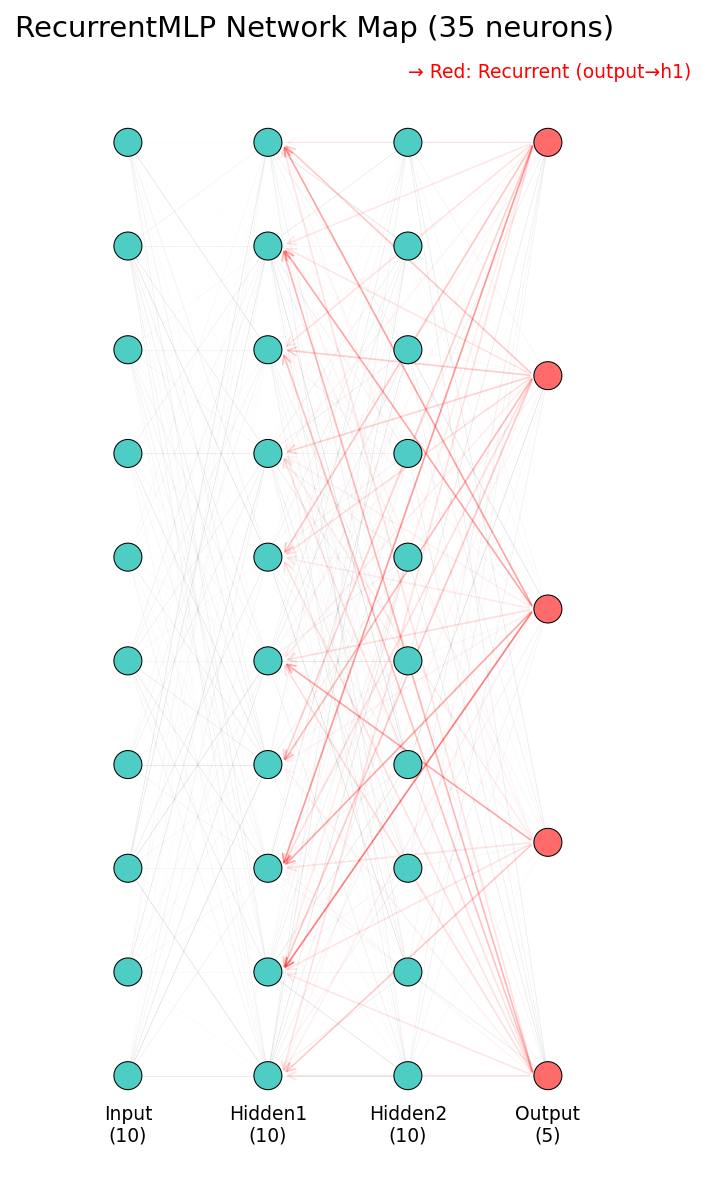
\includegraphics[width=0.7\linewidth]{../results/network_map.png}
\caption{Architecture of the 35-neuron RecurrentMLP. The recurrent feedback pathway (output $\to$ hidden layer~1) is shown in red. All weights are directly accessible and inspectable.}
\label{fig:architecture}
\end{figure}

\subsection{Task: Static Pattern Classification with Self-Correction}

To isolate self-reference from memory, we used a static input task. Five prototype patterns were defined over 10 input dimensions: each class $k$ activates dimensions $2k$ and $2k{+}1$ with amplitude 1.0, and adjacent class dimensions with amplitude 0.3 (inter-class ambiguity). Input samples were generated by adding Gaussian noise ($\sigma = \text{noise\_level}$) to the prototype. On each trial, the network receives the same noise-corrupted pattern at every timestep $t = 1, 2, 3$. The task is 5-class classification. Because the input is identical at every timestep, the recurrent loop cannot serve as a memory pathway---its only function is to allow the network to observe and revise its own prior output.

This design cleanly separates two potential roles of recurrence: memory (carrying information about past inputs) and self-correction (carrying information about past outputs). In our task, only the latter is possible.

\subsection{Training and the Conditions for Induction}

Training used full-batch gradient descent with learning rate 0.01 for 500 epochs on 200 training samples (200 held-out test samples), with $T = 3$ timesteps per trial. Backpropagation through time was implemented as a 3-step unroll, with numerical gradient checking (relative error threshold $10^{-4}$) to verify correctness. Numerical gradient checking on a representative model (seed=0) yielded maximum relative errors of $6.57 \times 10^{-8}$ (static) and $1.48 \times 10^{-7}$ (variable noise) across all weight matrices, well below the $10^{-4}$ acceptance threshold.

Two modifications appeared important for reliably inducing self-correction in the reported setup:

\textbf{Time-weighted loss.} The per-timestep loss $L(t)$ is softmax cross-entropy between the output logits and the one-hot target. The total loss is weighted across timesteps as $L = w_1 \cdot L(t{=}1) + w_2 \cdot L(t{=}2) + 1.0 \cdot L(t{=}3)$. With uniform weighting ($w_1 = w_2 = 1/3$), the network optimizes for immediate accuracy at $t{=}1$ and has no incentive to develop an iterative correction strategy. Setting $w_1 = 0.0$ grants the network temporal freedom: ``your initial guess carries no penalty; only the final answer matters.'' This creates optimization pressure to use the feedback loop for refinement.

\textbf{Temperature scaling.} Without temperature scaling, output logits quickly exceed $\pm 3$, saturating the $\tanh$ feedback function and driving the gradient of the recurrent weights to near zero. Setting $\tau = 2.0$ prevents saturation and maintains gradient flow through the feedback pathway.

The failure to develop self-correction under uniform loss and unscaled feedback is itself informative: it demonstrates that the phenomenon depends on learning conditions, not latent capacity.

\subsection{Ablation Design}

We employed ten evaluation conditions (Baseline plus nine ablation/control conditions) to isolate the contribution of self-referential feedback:

\textbf{Baseline}: The fully trained recurrent model, evaluated normally.

\textbf{Group~A (Recurrent ablation)}: All recurrent weights set to zero post-training. The feedback pathway is structurally intact but carries no signal. This tests whether self-correction depends on the recurrent loop.

\textbf{Group~B1 (Random ablation)}: The same number of weights (50) randomly zeroed across all weight matrices. Repeated 30 times per model with different random seeds. This controls for the general effect of removing an equal number of parameters.

\textbf{Group~B2 (Structured ablation)}: The h2-to-output weight matrix zeroed entirely, removing a major feedforward pathway. This controls for the effect of removing an entire structural pathway (as opposed to the scattered damage of B1).

\textbf{Group~C1 (Permutation feedback)}: The recurrent connections are preserved, but the feedback vector is element-wise permuted at each timestep. This maintains the exact distribution, norm, and dimensionality of the feedback signal while destroying its coordinate-structured identity---the network receives a scrambled version of its own output. The permutation was independently resampled at each timestep within each trial, using a per-model random seed. We refer to this as the ``non-veridical feedback'' or ``fake mirror'' condition.

\textbf{Group~C2 (Clone feedback)}: The recurrent connections are preserved, and the feedback is replaced with the output of a different model trained with identical architecture and procedure but a different random seed. Each target model (seed 0--9) is paired with a separately trained donor model (seed 100--109), ensuring full statistical independence between pairs. The clone's output is well-formed, in-distribution, and a valid classification output---but it is not the model's own. This condition controls for marginal-distribution mismatch: the clone's output has valid statistics (correct dimensionality, plausible magnitudes, trained output geometry), so any remaining degradation indicates trajectory-level specificity rather than distributional artifact. As a robustness check, we also tested a data-matched variant in which each donor model was trained on the exact same empirical data (identical noise realizations) as its target, differing only in weight initialization, to isolate the pure effect of initialization trajectory from any data-distribution confound.

\textbf{Group~C2-aligned (Affine-aligned clone feedback)}: To disentangle linear representation misalignment from model-specific geometric incompatibility in the C2 condition, we fitted a learned affine transform from donor logits to target logits. Both models were run with self-feedback on calibration data (target's training set, 200 samples $\times$ 3 timesteps $=$ 600 logit pairs); a least-squares regression $\text{target\_logit} \approx W \cdot \text{donor\_logit} + b$ (30 parameters: $5 \times 5$ weight matrix $+$ 5 bias) was fitted and applied to donor outputs before injection during evaluation on the held-out test set.

\textbf{Group~D (Feedforward baseline)}: A network trained from scratch with no recurrent connections. This tests whether recurrence was necessary for the observed behavior to develop.

\textbf{Group~D$'$ (Parameter-matched feedforward)}: A feedforward network with an additional skip connection from input to output (50 weights), matching the total parameter count of the recurrent model. This addresses the possibility that the recurrent model's advantage is simply due to having more parameters.

\textbf{Group~D$''$ (Compute-matched feedforward)}: A deep feedforward network with 6 hidden layers of 10 neurons each (Input(10) $\to$ H1(10) $\to$ \ldots $\to$ H6(10) $\to$ Output(5)), matching the computational depth of the recurrent model's 3-timestep unroll (3 timesteps $\times$ 2 hidden layers $=$ 6 layer traversals). This has 715 parameters (vs.\ Baseline 325) and approximately 650 multiply-add operations (vs.\ Baseline $\sim$900 MACs across 3 timesteps). This addresses the possibility that the recurrent model's advantage comes from additional computation rather than from feedback content.

\subsection{Variable-Noise Task}
\label{sec:vn}

To move beyond the static-input setting---where removing recurrence deterministically produces zero gain because no new information enters across timesteps---we introduce a variable-noise variant: at each timestep $t$, the network receives $x_t = \text{prototype}_k + \varepsilon_t$, where $\varepsilon_t \sim \mathcal{N}(0, \sigma^2 I)$ is independently sampled. Note that a stateless model under i.i.d.\ inputs still has expected gain of zero by symmetry; the VN task's value is not that it changes the Group~A baseline, but that it provides multiple independent observations of the same class across timesteps, creating an opportunity for temporal evidence accumulation that the static-input setting cannot offer. The task largely preserves the separation of memory and self-correction: although the class identity is constant, prior outputs are functions of earlier noisy inputs, so recurrence may carry some indirect past-input information. Models were retrained under variable noise with the same hyperparameters ($w_1{=}0.0$, $w_2{=}0.2$, $\tau{=}2.0$, 500 epochs). Ten donor models (seeds 100--109) were also retrained for the C2 condition. Under variable noise, the donor and target networks were driven by the same per-timestep noisy input sequence during evaluation, ensuring that any difference in output is attributable to model identity rather than input variation.

\subsection{Feedback Interpolation}
\label{sec:interpolation}

To map the continuous boundary of feedback-contract specificity, we swept the interpolation coefficient $\alpha \in \{0.0, 0.1, \ldots, 1.0\}$ in:
\[
\text{feedback}_t = \alpha \cdot y_{\text{self},t-1} + (1-\alpha) \cdot y_{\text{other},t-1}
\]
with three contamination types: Self--Zero ($y_\text{other} = 0$), Self--Shuffle ($y_\text{other} = \text{permuted}\; y_\text{self}$), and Self--Clone ($y_\text{other} = \text{clone output}$). All 10 model pairs were evaluated at noise $= 0.5$. This provides graded evidence for whether the feedback contract is ``hard'' (sharp threshold) or ``soft'' (linear degradation).

\subsection{Mechanistic Analysis}
\label{sec:mechanistic}

To exploit the glass-box transparency afforded by the 35-neuron architecture, we performed three mechanistic analyses on the static-input models:

\textbf{(a) Activation logging and trial classification.} For each of the 10 models $\times$ 200 test samples $\times$ 3 timesteps, we recorded all internal activations (pre/post-activation at each layer, feedback signals, recurrent contributions). Trials were classified as \emph{corrected} (wrong at $t{=}1$, correct at $t{=}3$), \emph{stable correct}, \emph{stable incorrect}, or \emph{over-corrected} (correct at $t{=}1$, wrong at $t{=}3$).

\textbf{(b) Hidden-state trajectory analysis.} Hidden Layer~1 activations (10-dim) were projected into a shared 2-component PCA space (fitted on Baseline $t{=}1$ activations). Trajectories ($t{=}1 \to t{=}2 \to t{=}3$) were plotted by trial category and compared across Baseline and C2 conditions.

\textbf{(c) Clone feedback geometric analysis.} For each trial, we computed the self-feedback $W_\text{rec}$ contribution ($\tanh(y_\text{self}/\tau) \cdot W_\text{rec}$) and clone-feedback $W_\text{rec}$ contribution ($\tanh(y_\text{clone}/\tau) \cdot W_\text{rec}$), measured their cosine divergence, and correlated divergence with correction outcome.

\subsection{Neuron Importance Analysis}

To quantify the contribution of individual neurons to pattern recognition and self-correction, we used decoupled single-neuron knockout analysis. For Hidden Layer~1 neurons (which receive both feedforward and recurrent input), intelligence and correction were measured separately: (a)~intelligence importance was measured by zeroing only the feedforward incoming weights ($W_\text{ih1}$ column + bias), observing the drop in $t{=}1$ accuracy ($\Delta\text{acc}_{t1}$); (b)~correction importance was measured by zeroing only the recurrent incoming weights ($W_\text{rec}$ column), observing the drop in correction gain ($\Delta\text{gain}$). This decoupling prevents a confound where feedforward-critical neurons appear artificially important for correction simply because destroying their feedforward pathway also collapses the correction baseline. For Hidden Layer~2 neurons (which have no direct recurrent input), full knockout was used for both measures; we note that the intelligence-correction confound may still exist for these neurons. This analysis was performed on a single trained model (seed=0, noise=0.5) to generate a per-neuron importance heatmap.

\subsection{Statistical Design}

All experiments were conducted across 10 independently initialized models (seeds 0--9). Groups B1 and C1 were repeated 30 times per model with different ablation/permutation seeds. Group C2 paired each target model (seed 0--9) with an independently trained donor model (seed 100--109). The primary measure was \textbf{correction gain}: accuracy at $t{=}3$ minus accuracy at $t{=}1$. Secondary measures included recurrent contribution norm ($\|\tanh(y_{t-1}/\tau) \cdot W_\text{rec}\|$) and step delta ($\|y_t - y_{t-1}\|$). For B1 and C1, the 30 repeats were averaged within each model before inference; the inferential unit is the model ($N{=}10$), not the repeat.

The pairing structure differs by group type: Groups A, B1, C1, and C2 are post-hoc interventions on the same trained model (within-model pairing); Groups D, D$'$, and D$''$ are separately trained seed-matched controls (matched-design pairing). B2 was excluded from the primary correction family a priori because its catastrophic feedforward degradation renders correction gain comparison uninformative. Under static input, D/D$'$/D$''$ produce gain $= 0.000$ by structural necessity (no recurrence, no new input); these are presented as structural controls confirming the task design, not as inferential tests, and are excluded from the Holm-Bonferroni family. The primary Holm-Bonferroni family for static-input comparisons thus consists of $m = 4$ tests: Baseline vs.\ \{A, B1, C1, C2\}. The secondary family (C1-vs-A and C2-vs-A) was pre-specified to test whether non-veridical feedback is worse than absent feedback.

The mean train-test accuracy gap at $t{=}3$ was $+0.040$ (static) and $+0.050$ (variable noise), indicating modest overfitting consistent with the small sample size (200 training samples). Full per-seed gaps are reported in the supplement.

Significance was assessed with exact Wilcoxon signed-rank tests on paired model-level means ($2^{10} = 1{,}024$ sign assignments enumerated), with Holm-Bonferroni correction for the primary family of comparisons. 95\% bootstrap confidence intervals (10,000 resamples, percentile method) are reported as descriptive summaries. For paired comparisons, the 10 model-level paired differences were resampled as a unit to preserve pairing structure; the exact Wilcoxon $p$-values are the primary inferential quantities. Noise level was set to 0.5 for the primary analysis, with a full sweep across $[0.1, 0.2, 0.3, 0.5, 0.7, 1.0]$.

\subsection{Robustness Analysis}
\label{sec:robustness_analysis}

To address potential concerns about parameter sensitivity, we conducted a hyperparameter sweep across 80 configurations: $w_1 \in \{0.0, 0.1, 0.2, 0.3\}$, $w_2 \in \{0.1, 0.2, 0.3, 0.5\}$, $\tau \in \{1.0, 1.5, 2.0, 3.0, 5.0\}$, with 10 independent models per configuration (800 total experiments). For the purpose of mapping the grid, we used a lenient heuristic to flag configurations showing self-correction: mean gain $> 0$ with at least 60\% of models showing positive gain. This criterion is deliberately liberal (a sign test at 6/10 yields $p \approx 0.38$) and is intended only for exploratory grid characterization, not as a formal significance test; the primary statistical claims rest on the exact Wilcoxon tests reported in Section~\ref{sec:results}.

% ============================================================
\section{Results}
\label{sec:results}
% ============================================================

\subsection{Variable-Noise Task (Primary Experiment)}
\label{sec:vn_results}

Under variable noise ($x_t = \text{prototype} + \varepsilon_t$, independent per timestep), the Baseline model achieved a correction gain of $\mathbf{+0.151 \pm 0.046}$ (mean $\pm$ SD, $N{=}10$), with a 95\% bootstrap CI of $[+0.121, +0.179]$. This is numerically 3.6$\times$ larger (descriptive ratio; no formal cross-task comparison was conducted) than the static-input gain ($+0.042$), consistent with a greater benefit from iterative refinement when each timestep provides a new noisy observation of the same underlying pattern.

\textbf{Group~A (recurrent ablation)} produced gain $= +0.008 \pm 0.045$---not significantly different from zero (Wilcoxon signed-rank vs.\ 0: $p = 0.754$, 5/10 models positive). Under i.i.d.\ inputs, a stateless model has expected gain of zero by symmetry, so Group~A's near-zero gain is the expected statistical baseline. The informative contrast is with the Baseline: the recurrent model achieves gain $= +0.151$ by accumulating evidence across timesteps---a capability that requires temporal integration through the feedback pathway.

\textbf{Group~C1 (shuffled feedback)} produced gain $= -0.068 \pm 0.087$ (CI: $[-0.123, -0.016]$), replicating the fake mirror effect under variable noise.

\textbf{Group~C2 (clone feedback)} produced gain $= -0.018 \pm 0.100$ (CI: $[-0.074, +0.048]$). While the CI includes zero for C2's own gain, the paired comparison against Baseline is maximally significant ($T = 0.0$, $p = 0.002$ raw, all 10 models show Baseline $>$ C2).

All three primary comparisons (Baseline vs.\ A, C1, C2) reached the resolution limit of the $N{=}10$ exact test ($T = 0.0$), with Holm-Bonferroni corrected $p = 0.00586$ for all three ($m = 3$ family; all three raw $p = 0.001953$, and Holm's monotonic step-down yields a common adjusted value). All significant at $\alpha = 0.01$. Paired difference bootstrap CIs (10,000 resamples, percentile method on 10 model-level paired differences): Baseline $-$ A $= +0.143$ $[+0.110, +0.181]$, Baseline $-$ C1 $= +0.219$ $[+0.163, +0.278]$, Baseline $-$ C2 $= +0.168$ $[+0.124, +0.203]$. Endpoint accuracies: Baseline $t{=}1 = 0.685 \pm 0.066$, $t{=}3 = 0.836 \pm 0.074$; Group~A $t{=}1 = 0.685 \pm 0.066$, $t{=}3 = 0.694 \pm 0.061$.

Under variable noise, the gain across noise levels peaked at noise $= 0.5$ (Baseline $+0.151$) and decreased at both extremes. Group~A fluctuated around zero at all noise levels.

\subsection{Static-Input Results}

Under static input (the same noisy pattern repeated at every timestep), the Baseline achieved a correction gain of $+0.042 \pm 0.029$ (CI: $[+0.023, +0.059]$). The primary inferential evidence comes from the VN results (\S\ref{sec:vn_results}); the static setting serves as the controlled special case where memory and self-correction are cleanly separated, enabling the exploratory mechanistic analyses in \S\ref{sec:trajectory_results}--\ref{sec:wrec_results}. Under static input, Group~A gain $= 0.000$ is structurally guaranteed; the non-trivial findings are Baseline's positive gain (learned) and C1/C2's negative gain (active interference). Paired difference bootstrap CIs: Baseline $-$ A $= +0.042$ $[+0.023, +0.059]$, Baseline $-$ C1 $= +0.106$ $[+0.074, +0.139]$, Baseline $-$ C2 $= +0.101$ $[+0.062, +0.148]$.

\subsection{Ablation Results}

\textbf{Recurrent ablation (Group~A)}: Correction gain dropped to exactly $0.000 \pm 0.000$ (structurally guaranteed under static input). Accuracy at $t{=}1$ was unchanged ($0.698 \pm 0.054$), confirming the ablation targets only the correction mechanism. The paired Wilcoxon test against Baseline yielded corrected $p = 0.064$ (Holm-Bonferroni, $m = 4$); this marginally non-significant result reflects the small and variable Baseline gain under static input (1/10 models negative), not uncertainty about the ablation effect, which is structurally guaranteed. Under variable noise, where the comparison is empirically meaningful, all three primary comparisons are significant at $p < 0.006$ (\S\ref{sec:vn_results}). Recurrent contribution norm ($2.163 \to 0.000$) and step delta ($1.162 \to 0.000$) both dropped to zero.

\textbf{Random ablation (Group~B1)}: Mean gain $= -0.004 \pm 0.016$. Accuracy at $t{=}1$ dropped substantially ($0.515 \pm 0.048$), indicating general degradation. The correction mechanism was also lost, but this is confounded by the overall performance collapse.

\textbf{Structured ablation (Group~B2)}: The h2-to-output pathway ablation completely severed the hidden layers from the output, causing catastrophic degradation to chance-level accuracy ($t{=}1 = 0.199 \pm 0.032$). This serves as a sanity check rather than a nuanced structural ablation: it confirms that destroying the entire predictive pathway is qualitatively different from the targeted recurrent ablation in Group~A. B2 was excluded from the Holm-Bonferroni correction family for this reason.

\textbf{Feedforward controls (Groups~D, D$'$, D$''$)}: Under static input, all three feedforward variants produced correction gain $= 0.000 \pm 0.000$ (structurally guaranteed). Their $t{=}1$ accuracies---D: $0.746 \pm 0.067$, parameter-matched D$'$: $0.822 \pm 0.031$, compute-matched D$''$ (6 layers): $0.600 \pm 0.130$---show that additional parameters (D$'$) improve pattern recognition and additional depth (D$''$) does not, but neither produces self-correction without recurrence. Under variable noise, D/D$'$/D$''$ were retrained and still showed gain $\approx 0$ (D: $-0.011 \pm 0.047$, D$'$: $-0.000 \pm 0.032$, D$''$: $+0.010 \pm 0.035$)---as expected for stateless models under i.i.d.\ inputs. Neither additional parameters (D$'$) nor additional computational depth (D$''$) enable evidence accumulation without recurrent feedback.

Table~\ref{tab:main} summarizes all experimental conditions.

\begin{table}[t]
\caption{Main results at noise level 0.5 (mean $\pm$ SD across $N{=}10$ models). Correction gain $=$ acc($t{=}3$) $-$ acc($t{=}1$). $p$-values are Holm-Bonferroni corrected ($m{=}4$: Baseline vs.\ A, B1, C1, C2). D/D$'$/D$''$: structural controls (gain $= 0$ by design). $^\dagger$Marginally non-significant; A gain $= 0$ is structurally guaranteed under static input.}
\label{tab:main}
\centering
\begin{tabular}{@{}lccccc@{}}
\toprule
Group & acc($t{=}1$) & acc($t{=}3$) & Gain & 95\% CI & Corr.\ $p$ \\
\midrule
\textbf{Baseline}   & $.698 \pm .054$ & $.739 \pm .055$ & $\mathbf{+.042}$ & $[+.023, +.059]$ & --- \\
A (Recurrent cut)    & $.698 \pm .054$ & $.698 \pm .054$ & $.000$           & $[.000, .000]$   & .064$^\dagger$ \\
B1 (Random cut)      & $.515 \pm .048$ & $.511 \pm .037$ & $-.004$          & $[-.013, +.006]$ & .027 \\
B2 (Structural cut)  & $.199 \pm .032$ & $.199 \pm .032$ & $.000$           & ---              & --- \\
C1 (Shuffled fb.)    & $.698 \pm .054$ & $.634 \pm .041$ & $\mathbf{-.064}$ & $[-.095, -.035]$ & .008 \\
C2 (Clone fb.)       & $.698 \pm .054$ & $.639 \pm .081$ & $\mathbf{-.059}$ & $[-.102, -.016]$ & .008 \\
D (Feedforward)      & $.745 \pm .067$ & $.745 \pm .067$ & $.000$           & ---              & \emph{struct.} \\
D$'$ (Param-matched) & $.822 \pm .031$ & $.822 \pm .031$ & $.000$           & ---              & \emph{struct.} \\
D$''$ (Compute-matched) & $.600 \pm .130$ & $.600 \pm .130$ & $.000$ & --- & \emph{struct.} \\
\bottomrule
\end{tabular}
\end{table}

\subsection{The Fake Mirror Effect}

Group~C1 (permutation feedback) produced gain $= -0.064 \pm 0.048$ (CI: $[-0.095, -0.035]$)---not merely zero, but significantly \emph{negative}. Shuffled feedback actively degrades performance below the initial prediction, despite preserving the full recurrent architecture and feedback distribution.

Group~C2 (clone feedback) controls for the possibility that C1's degradation is an OOD artifact: the clone's output has valid marginal statistics but is not the model's \emph{own}. C2 produced comparable degradation: gain $= -0.059 \pm 0.069$ (CI: $[-0.102, -0.016]$, corrected $p = 0.008$). No significant difference between C1 and C2 was detected ($p = 0.846$, $N = 10$).

Both C1 and C2 are significantly worse than Group~A (no feedback, gain $= 0.000$) in the secondary comparison family: C1 vs A corrected $p = 0.008$, C2 vs A corrected $p = 0.065$ (marginally non-significant; raw $p = 0.064$). Non-veridical feedback actively degrades performance below the no-feedback baseline. We term this \emph{learned feedback-contract specificity}: the recurrent weights are co-adapted to the model's own output geometry, and foreign substitution---even with valid marginal statistics---degrades the correction mechanism. The boundary between model-specific contract violation and ordinary closed-loop co-adaptation remains an open question (\S4.6).

A data-matched clone (identical training data, different initialization) produced gain $= -0.054$ ($p = 0.006$ vs Baseline), confirming that the effect is driven by weight initialization trajectory, not data distribution. A cross-pairing analysis (100 donor-target pairings under VN) showed mean C2 gain $= -0.043 \pm 0.096$, with substantial donor variance (per-target SD: 0.05--0.12).

\subsection{Noise Dependence}

Under static input, the correction gain varied with noise level, peaking at noise $= 0.2$ (gain $\approx +0.099$) and declining at both lower and higher noise levels. At low noise (0.1), feedforward processing alone was sufficient, rendering self-correction unnecessary. At high noise (0.7--1.0), the signal was too degraded for correction to recover. The optimal zone---where self-correction provides the greatest advantage---occurs at intermediate difficulty: noise is high enough that initial predictions are frequently wrong but low enough that the underlying signal remains recoverable through iterative refinement.

\begin{figure}[t]
\centering
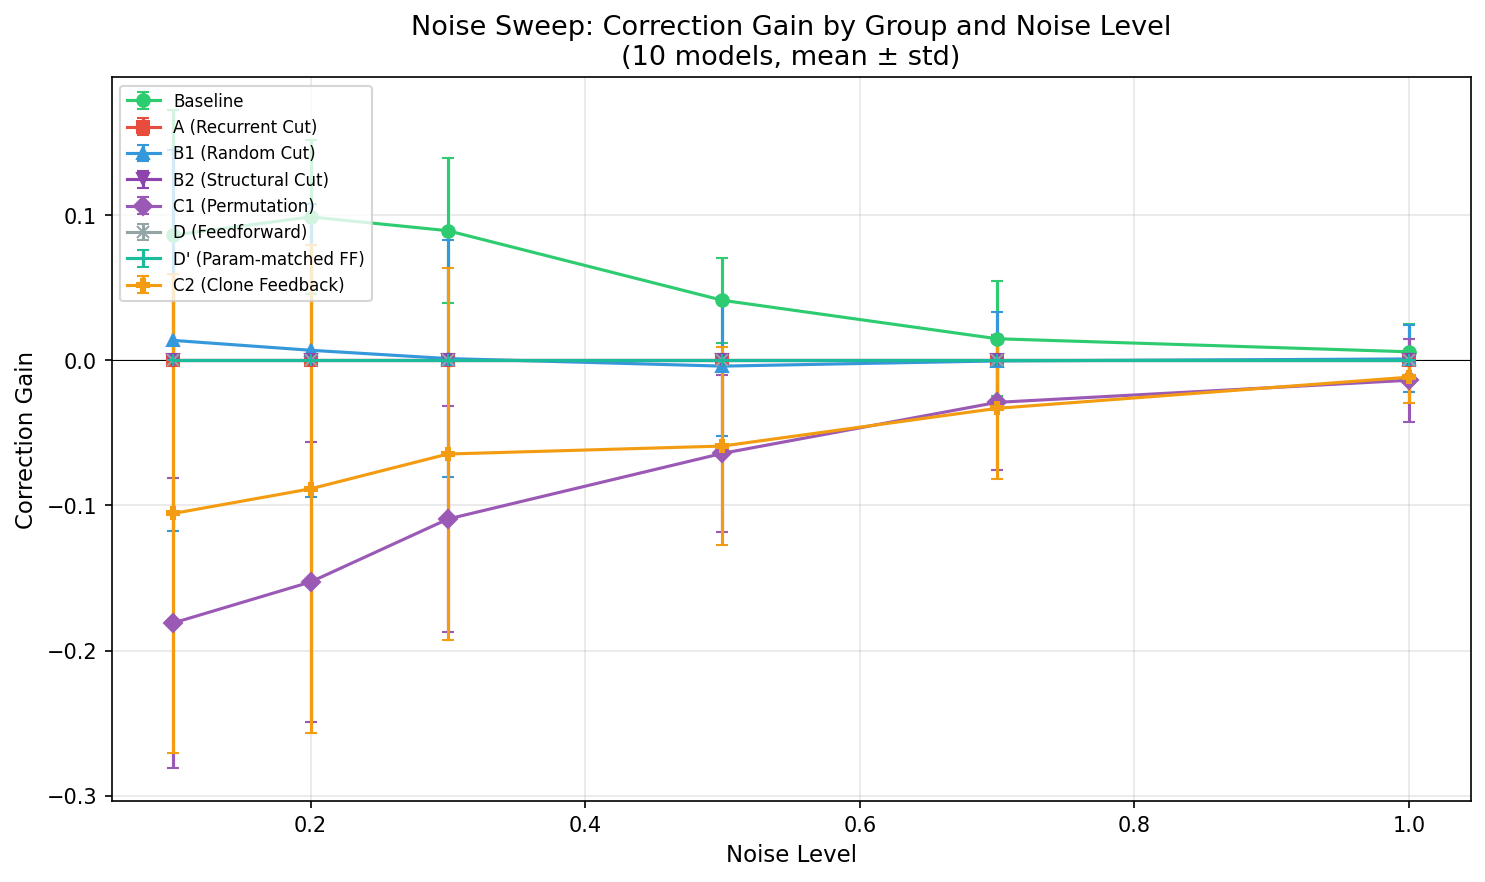
\includegraphics[width=0.8\linewidth]{../results/noise_sweep_curve.png}
\caption{Correction gain across noise levels for Baseline and ablation groups. Self-correction peaks at moderate noise ($\sigma = 0.2$) and declines at both extremes.}
\label{fig:noise}
\end{figure}

\subsection{Feedback Interpolation}
\label{sec:interpolation_results}

The interpolation sweep (\S\ref{sec:interpolation}) revealed a smooth, monotonic relationship between self-feedback fidelity ($\alpha$) and correction gain. There is no sharp threshold---degradation is smooth and roughly monotonic across the sampled $\alpha$ values, indicating that the feedback contract is ``soft'': the network degrades gracefully rather than collapsing suddenly.

Key quantitative landmarks (mean across 10 models, noise $= 0.5$; evaluated on a held-out test set distinct from the primary ablation experiment, yielding a Baseline gain of $+0.053$ on this sample vs.\ $+0.042$ in \S3.2---the difference reflects sampling variance across test sets):
\begin{itemize}
  \item $\alpha = 1.0$ (pure self): gain $= +0.053$ $[+0.019, +0.086]$ (Baseline on this test set)
  \item $\alpha = 0.5$ (half self): zero: $+0.053$ $[+0.026, +0.078]$, shuffle: $+0.039$ $[+0.010, +0.068]$, clone: $+0.031$ $[-0.001, +0.064]$---still positive
  \item $\alpha = 0.2$: zero: $+0.034$ $[+0.019, +0.048]$, shuffle: $+0.001$ $[-0.024, +0.027]$, clone: $-0.009$ $[-0.047, +0.030]$---zero-crossing region
  \item $\alpha = 0.0$ (no self): zero: $0.000$, shuffle: $-0.042$ $[-0.073, -0.008]$, clone: $-0.038$ $[-0.081, +0.004]$
\end{itemize}

(All brackets are 95\% bootstrap CIs, 10,000 resamples, $N{=}10$ models.)

The zero-crossing occurs at approximately $\alpha \approx 0.2$ for Self--Shuffle and $\alpha \approx 0.3$ for Self--Clone, meaning the clone signal requires more self-feedback to overcome---consistent with structured misdirection being harder to compensate than incoherent noise. The Self--Zero curve plateaus around $\alpha \approx 0.5$, suggesting that $\sim$50\% self-feedback is sufficient for near-maximum correction.

\begin{figure}[t]
\centering
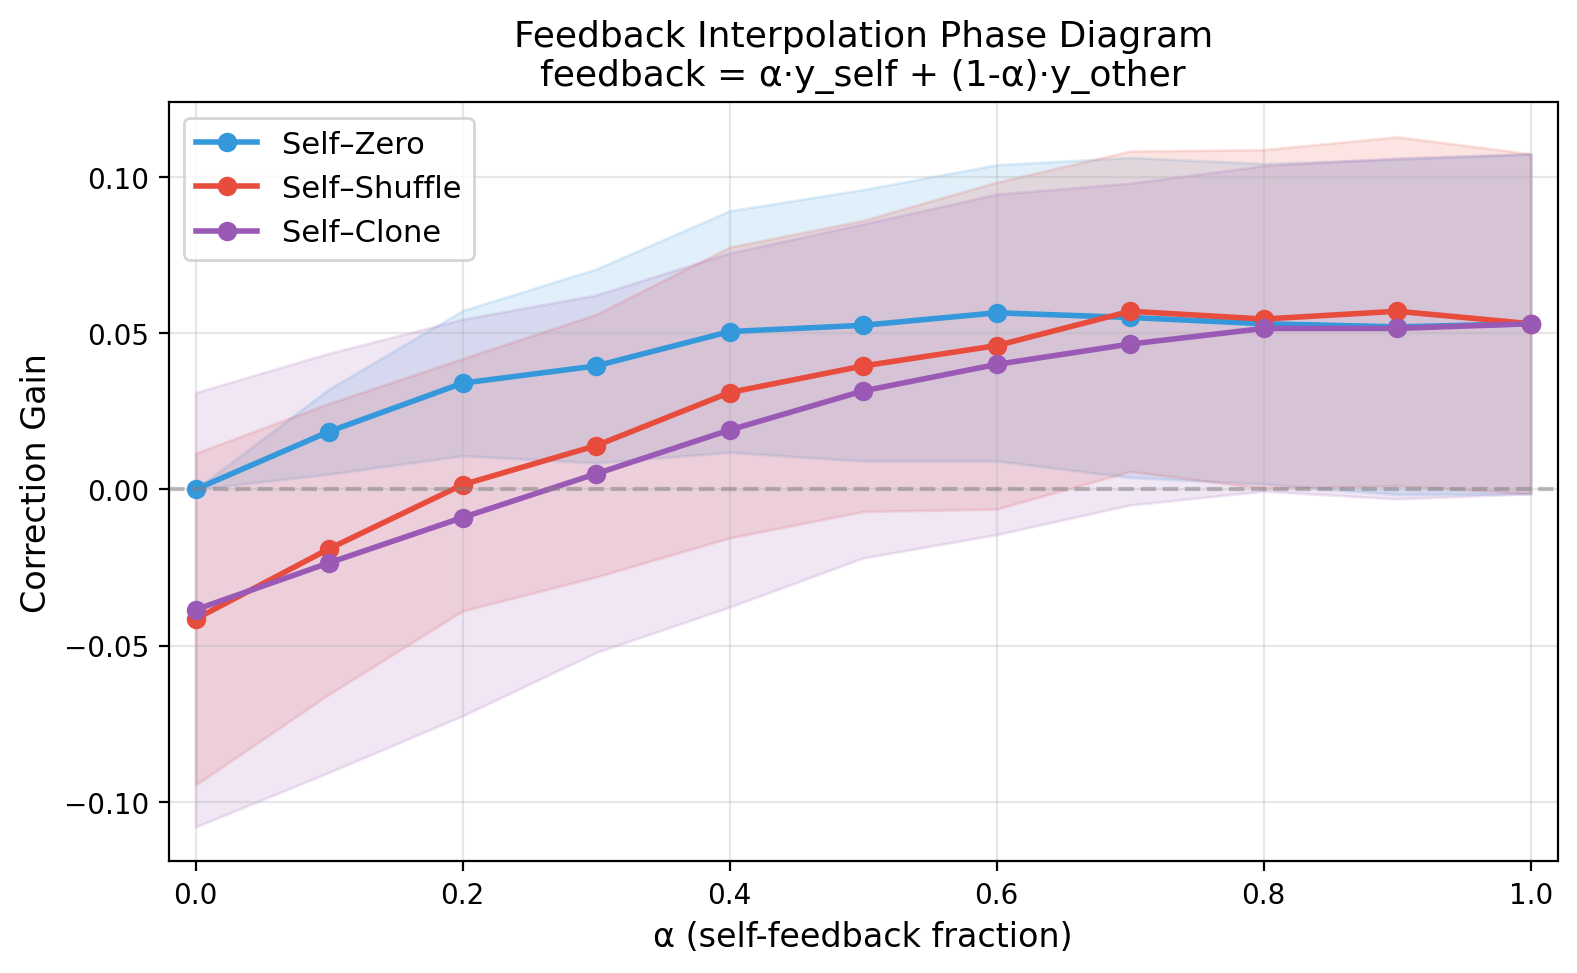
\includegraphics[width=0.8\linewidth]{../results/interpolation_phase.png}
\caption{Correction gain as a function of interpolation coefficient $\alpha$ for three contamination types. The smooth, monotonic degradation reveals a ``soft'' feedback contract.}
\label{fig:interpolation}
\end{figure}

\subsection{Mechanistic Analysis: Hidden-State Trajectories}
\label{sec:trajectory_results}

\emph{The following mechanistic analyses (\S\ref{sec:trajectory_results}--\ref{sec:wrec_results}) exploit the glass-box transparency of the 35-neuron architecture. These are conducted on the static-input models, where the primary statistical evidence is weaker than under variable noise (\S\ref{sec:vn_results}); the mechanistic results should be interpreted as exploratory characterizations of the correction mechanism, not as independent confirmatory tests.}

Across all 10 models (2,000 total test trials at noise $= 0.5$), trial classification revealed: corrected 236 (11.8\%), stable correct 1,258 (62.9\%), stable incorrect 376 (18.8\%), over-corrected 130 (6.5\%). The net gain (corrected minus over-corrected) is 106/2,000 $= 5.3$\%, consistent with the Baseline gain ($+0.042$ on the primary test set; $+0.053$ on the mechanistic analysis test set, which shares the same held-out data as the interpolation experiment).

PCA projection of Hidden Layer~1 activations (10-dim $\to$ 2-dim) reveals distinct trajectory patterns:
\begin{itemize}
  \item \textbf{Corrected trials} (Baseline): trajectories move toward class-appropriate regions between $t{=}1$ and $t{=}3$, consistent with the hidden state moving toward regions associated with correct classification.
  \item \textbf{Over-corrected trials} (Baseline): trajectories move away from the correct region---the feedback signal is occasionally misleading even when it is the model's own output.
  \item \textbf{C2 trials}: trajectories show comparable displacement magnitude but in misaligned directions, consistent with the clone feedback providing a coherent but incorrectly directed correction signal.
\end{itemize}

\begin{figure}[t]
\centering
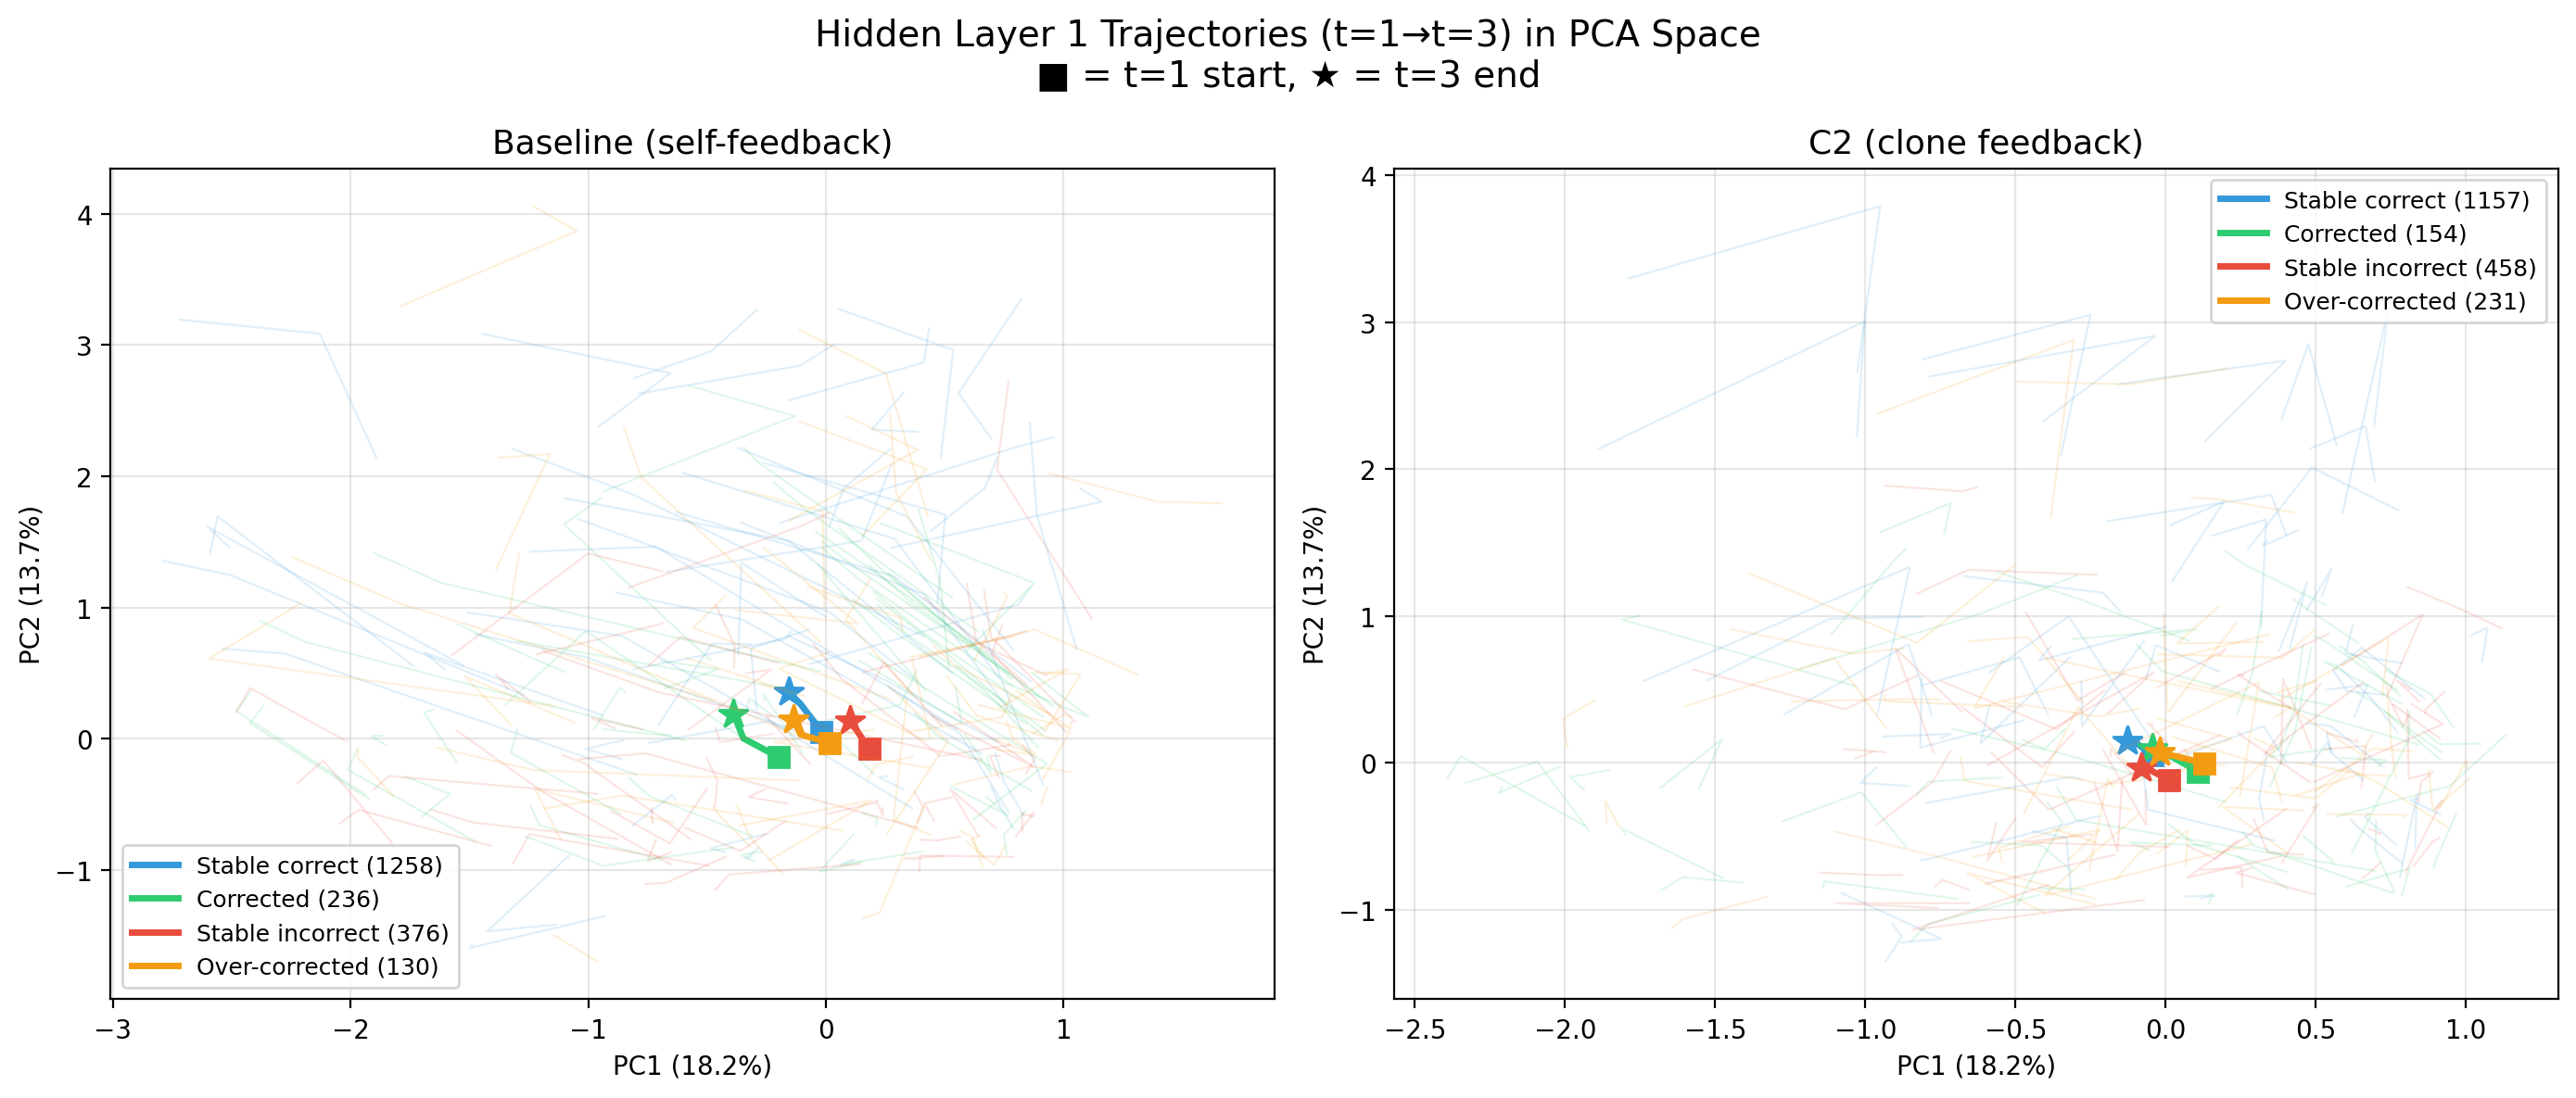
\includegraphics[width=0.8\linewidth]{../results/trajectory_hero.png}
\caption{PCA-projected hidden-state trajectories ($t{=}1 \to t{=}2 \to t{=}3$) for corrected, over-corrected, and C2 trials. Self-feedback steers corrected trials toward class centroids; clone feedback produces comparable displacement in misaligned directions.}
\label{fig:trajectory}
\end{figure}

\subsection{Wrong-Trajectory Control}
\label{sec:wrong_trajectory}

To distinguish model-specific feedback-contract specificity from ordinary state-conditional mismatch, we tested whether the \emph{same model's} output from a \emph{different trial} (matched on predicted class and $t{=}1$ correctness; when multiple candidates matched, one was selected uniformly at random using a fixed seed for reproducibility) also degrades performance. Under static input, self-wrong-trial gain $= +0.061 \pm 0.061$, nearly identical to self-current gain ($+0.053$, $p = 0.49$ for the difference), while clone gain $= -0.039 \pm 0.070$. The key comparison---self-wrong-trial vs.\ clone---shows mean difference $= +0.099$ ($p = 0.049$, uncorrected; this exploratory comparison was not part of the pre-specified Holm family). Under variable noise, the pattern is stronger: self-wrong-trial gain $= +0.138 \pm 0.053$ vs.\ clone gain $= -0.018 \pm 0.100$, difference $= +0.156$ ($p = 0.002$, uncorrected; consistent across all 10 model pairs). This suggests that foreign-model identity, not merely state-conditional mismatch, contributes to the C2 degradation: the network tolerates its own output from the wrong trial but not another model's output.

\subsection{Mechanistic Analysis: Clone Feedback Geometry}
\label{sec:geometry_results}

The cosine divergence between self and clone feedback $W_\text{rec}$ contributions at $t{=}2$ averaged $0.734 \pm 0.485$ across all 2,000 trials. To contextualize this value, we computed null baselines: isotropic norm-matched random vectors produced mean divergence $= 1.001 \pm 0.053$, same-class resampled self-feedback produced mean divergence $= 0.361 \pm 0.428$, and clone feedback produced $0.734 \pm 0.485$. The ordering---Resampled (0.361) $<$ Clone (0.734) $<$ Random (1.001)---reveals that clone feedback is more aligned than random noise but substantially less aligned than same-model same-class feedback. This contextualizes the 0.73 value as representing partial but insufficient alignment: the clone shares some structural similarity with the model's own output (they trained on similar tasks) but lacks the model-specific geometric properties needed for effective correction.

At the seed level, higher mean clone divergence correlated with lower C2 gain (Spearman $\rho = -0.61$, $p = 0.062$, $N = 10$), directionally consistent with angular misalignment as a contributing mechanism. The clone's output activates $W_\text{rec}$ in a direction that is angularly misaligned with what the model's learned correction strategy expects. This divergence operates at the continuous logit level, not at the discrete class level---even when self and clone outputs agree on the predicted class (same argmax), their continuous vectors produce meaningfully different $W_\text{rec}$ contributions.

To test whether this geometric misalignment is linearly correctable, we fitted a learned affine transform ($W \in \mathbb{R}^{5 \times 5}$, $b \in \mathbb{R}^5$; 30 parameters) from donor logits to target logits on calibration data (training set, 200 samples $\times$ 3 timesteps) and re-evaluated C2 gain on the held-out test set. The alignment quality was moderate ($R^2 = 0.449 \pm 0.053$ static, $0.465 \pm 0.104$ VN), confirming that the donor-to-target logit mapping is substantially non-linear. The affine-aligned C2 condition recovered a significant portion of the lost gain---static: C2-raw $= -0.059$, C2-aligned $= +0.010$, recovering 68\% of the Baseline-to-C2 gap; VN: C2-raw $= -0.030$, C2-aligned $= +0.062$, recovering 54\%---but remained significantly below Baseline in both settings (static: $p = 0.039$; VN: $p = 0.006$, Holm-Bonferroni corrected). The improvement from raw to aligned C2 was also significant (static: $p = 0.031$; VN: $p = 0.037$). This quantitative decomposition indicates that approximately 60\% of C2 degradation reflects linear representation misalignment (recoverable by affine transform), while the remaining ${\sim}40\%$ reflects non-linear, model-specific geometric incompatibility that persists even after optimal linear alignment.

\begin{figure}[t]
\centering
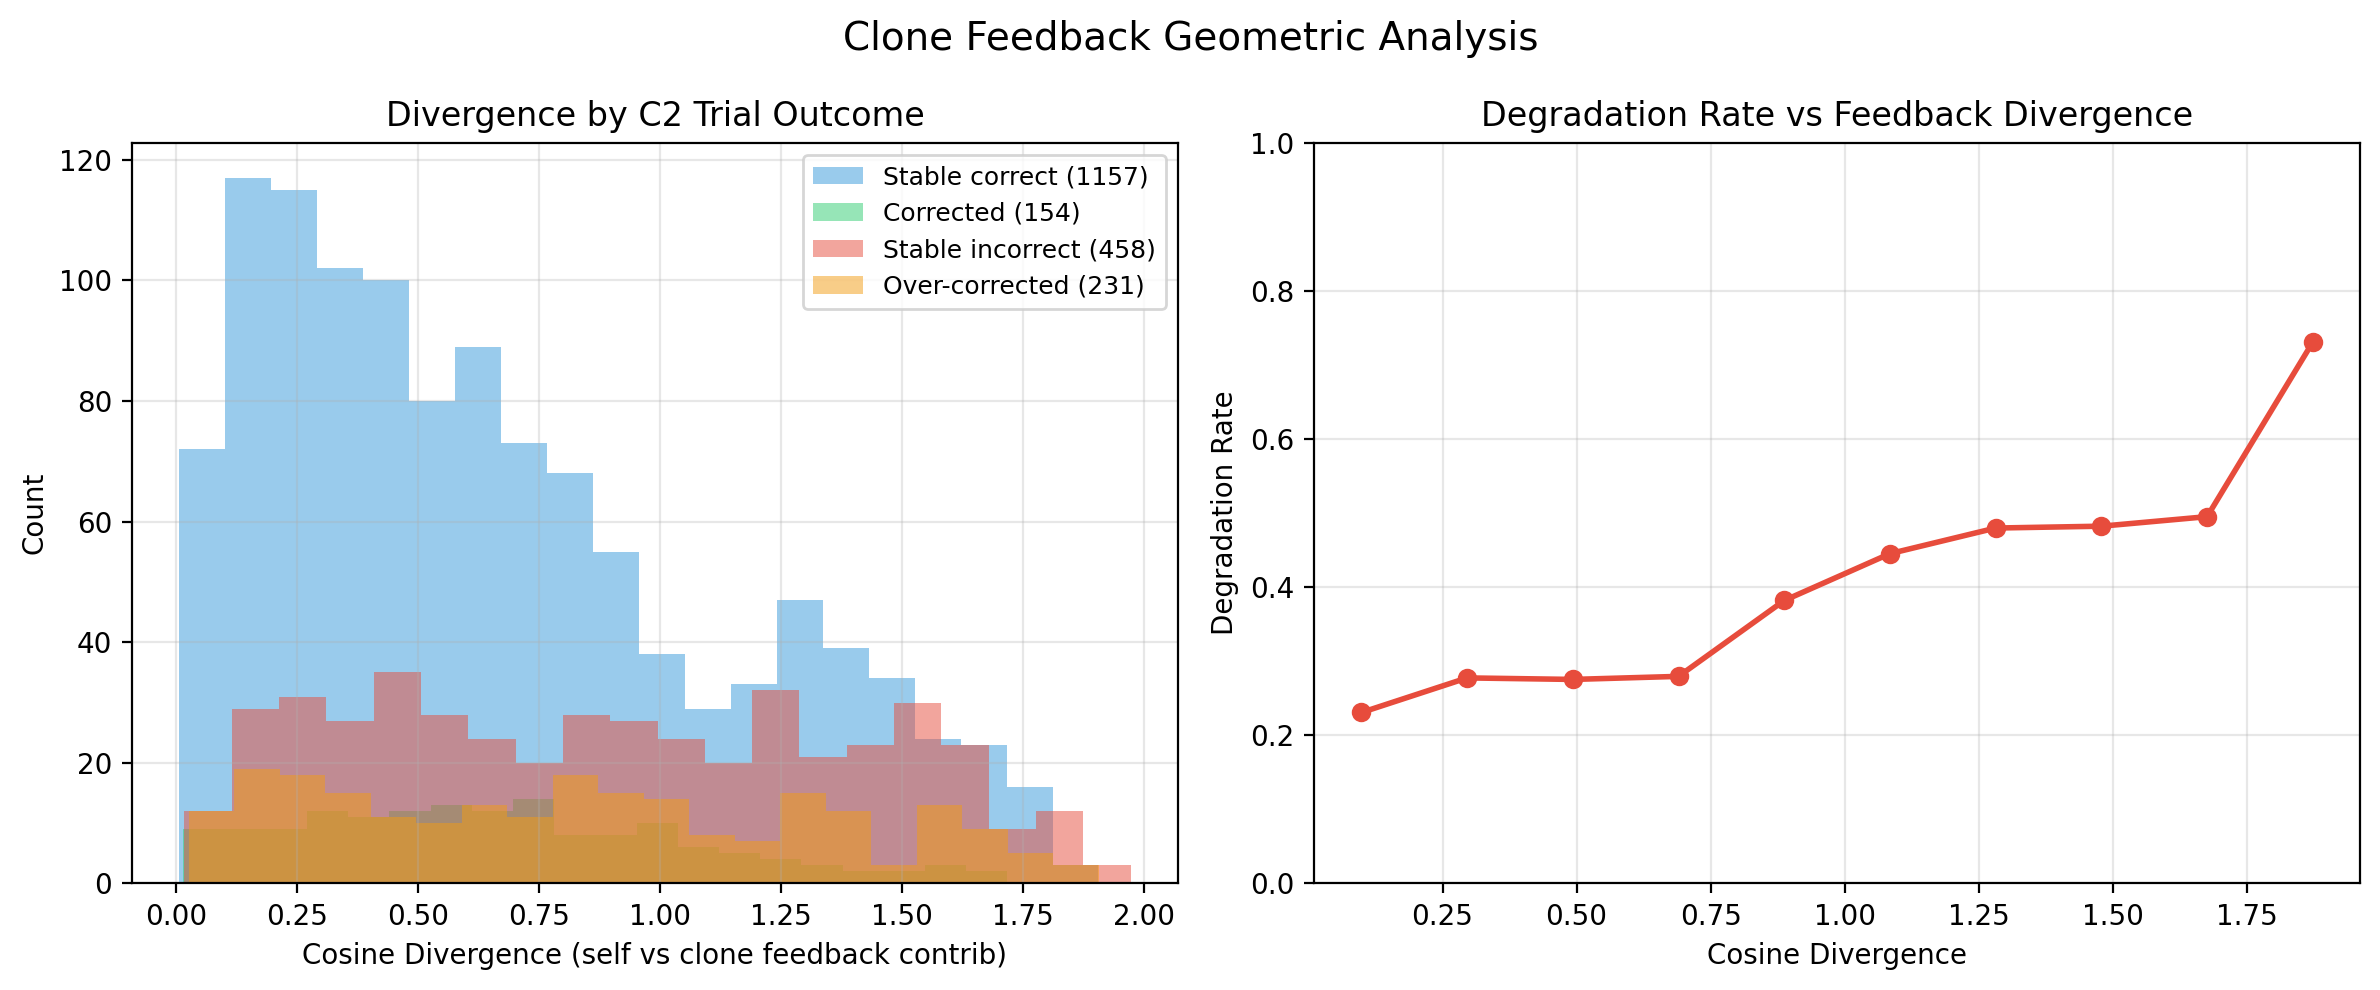
\includegraphics[width=0.8\linewidth]{../results/cosine_divergence.png}
\caption{Cosine divergence between self and clone $W_\text{rec}$ contributions. High divergence indicates angular misalignment in the feedback activation space.}
\label{fig:cosine}
\end{figure}

\subsection{$W_\text{rec}$ Structural Analysis}
\label{sec:wrec_results}

The recurrent weight matrix $W_\text{rec}$ ($5 \times 10$, output $\to$ hidden layer~1) showed moderate structural consistency across the 10 independently trained models: mean sign consistency $= 0.614$, minimum $= 0.300$. This indicates that $W_\text{rec}$ is neither fully interpretable (consistent across seeds) nor fully distributed (random across seeds), but occupies an intermediate regime where certain output-to-hidden connections are robustly signed while others depend on the specific training trajectory. This partial consistency is itself informative: it suggests that multiple distinct $W_\text{rec}$ configurations can implement effective self-correction, supporting the view that feedback-contract specificity operates at the model level rather than reflecting a single universal correction algorithm. No Hidden Layer~1 neurons became permanently inactive under Group~A ablation across all 10 models; activation fractions shifted by at most 12.3 percentage points (h1\_9: 60.7\% $\to$ 73.0\%), confirming that the ablation does not confound recurrent-pathway removal with ReLU dead-zone effects.

\begin{figure}[t]
\centering
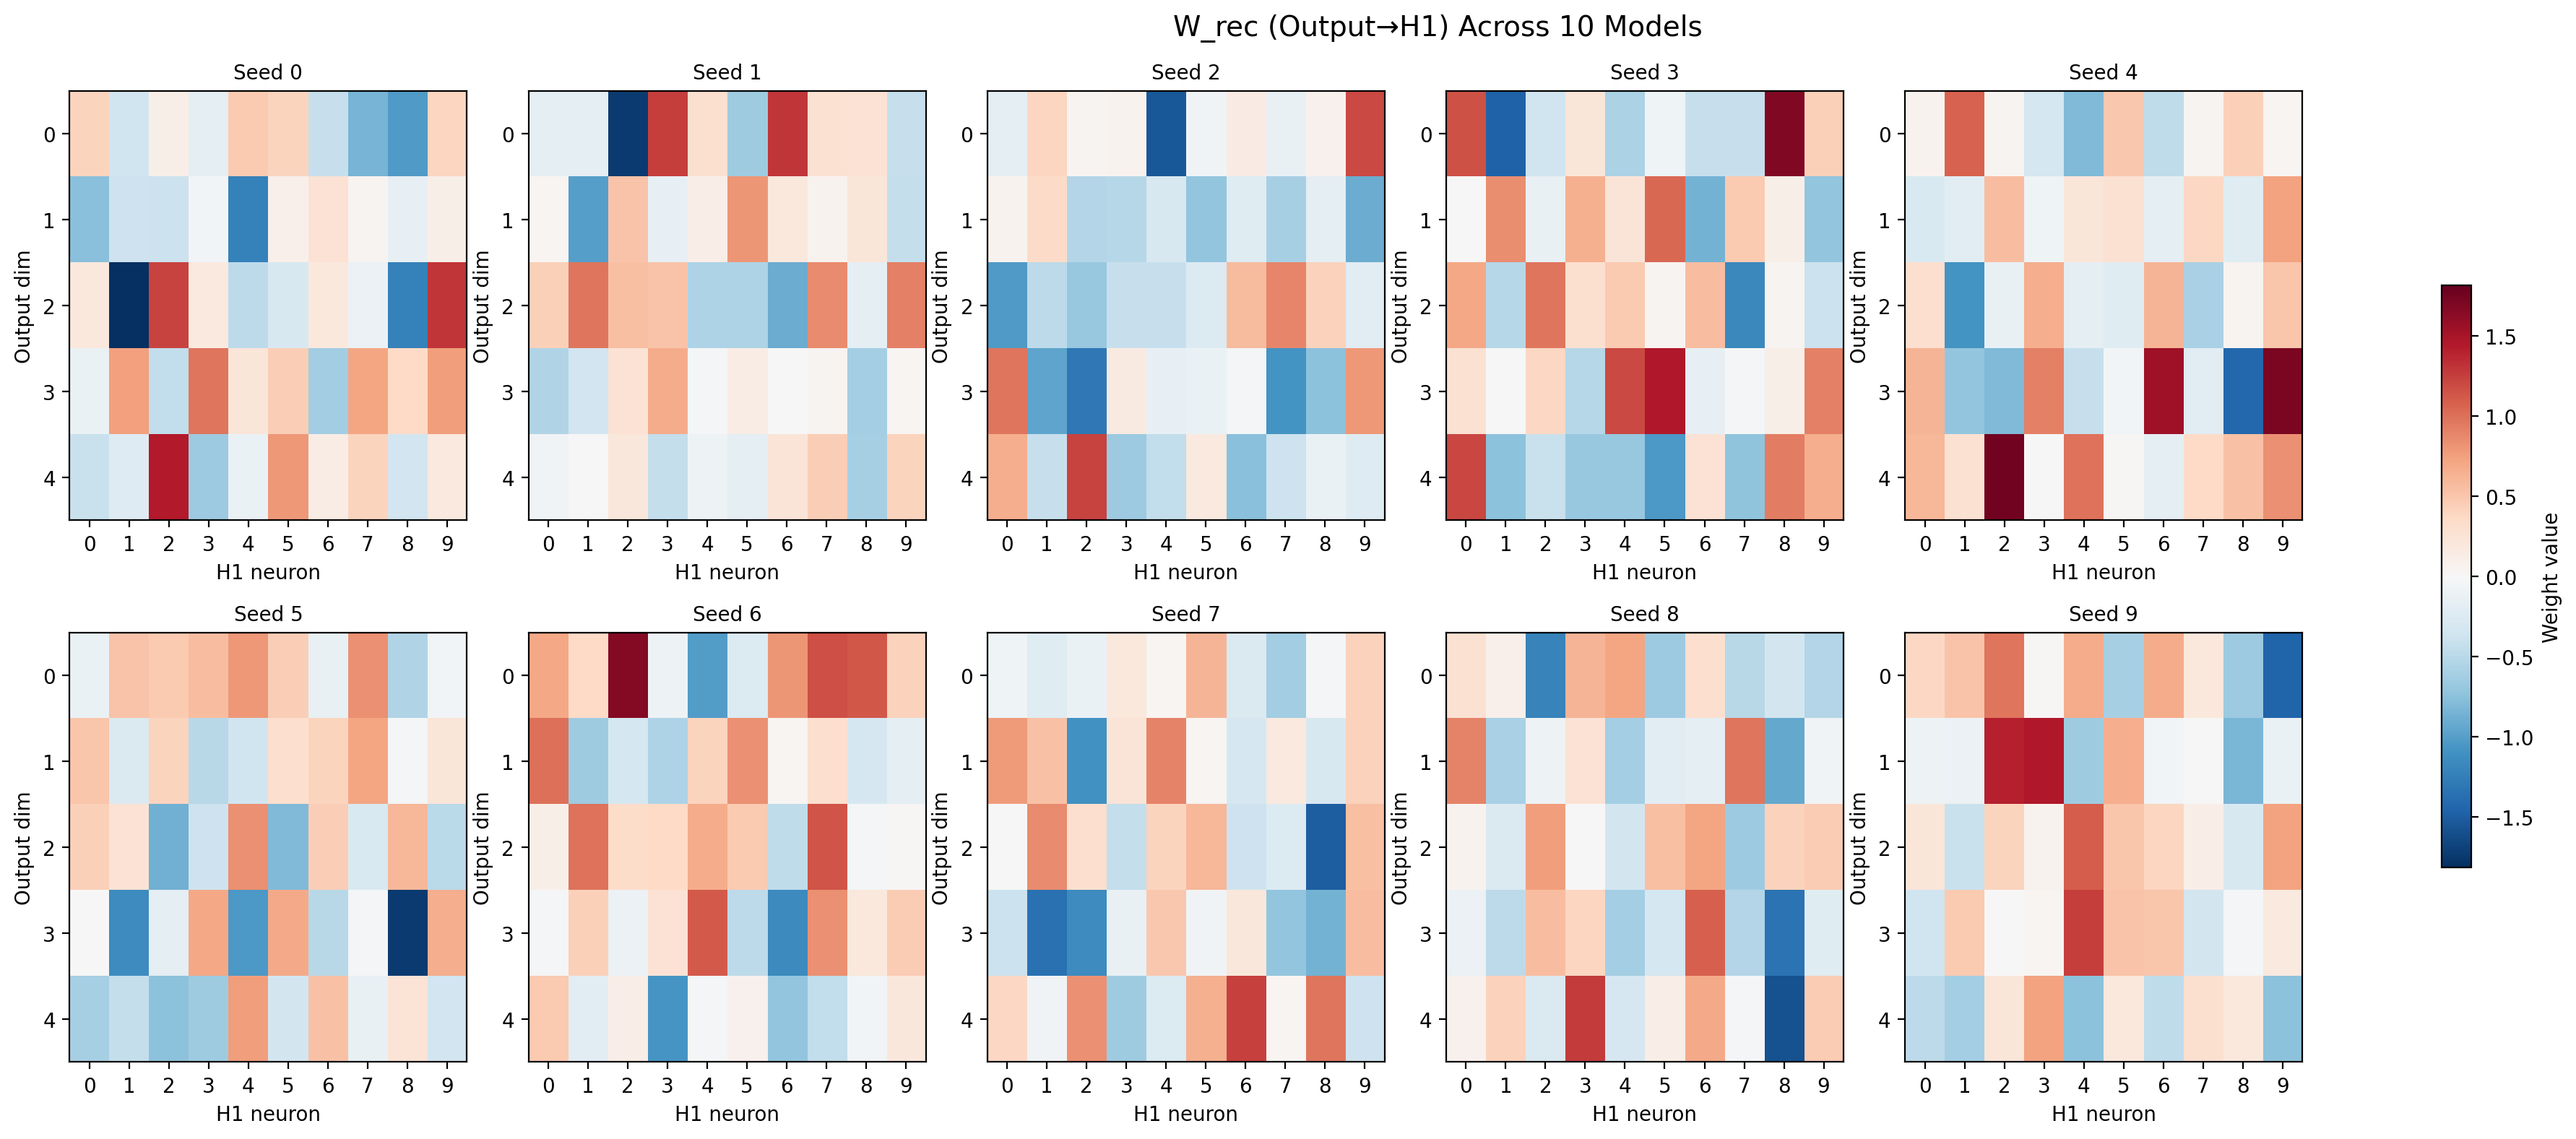
\includegraphics[width=0.8\linewidth]{../results/wrec_heatmap.png}
\caption{$W_\text{rec}$ heatmaps across 10 independently trained models. Moderate sign consistency (0.614) indicates model-specific rather than universal recurrent structure.}
\label{fig:wrec}
\end{figure}

\subsection{Neuron Overlap Analysis (Exploratory)}

Decoupled neuron importance analysis of Hidden Layer~1 (performed on a single model, seed=0)---where feedforward and recurrent contributions can be cleanly separated---revealed three functional groups: neurons important primarily for initial pattern recognition (intelligence-specialized, e.g., h1\_6), neurons whose recurrent input contributes primarily to self-correction (correction-specialized, e.g., h1\_8), and neurons important for both (shared, e.g., h1\_1, h1\_5, h1\_7). Notably, h1\_9 showed \emph{negative} correction importance ($-0.035$): removing its recurrent input \emph{improved} correction gain, suggesting that not all recurrent channels contribute positively. For Hidden Layer~2 (where decoupling is not possible without timestep masking), full knockout was used; the intelligence-correction confound should be noted when interpreting these values.

\subsection{Robustness}

The hyperparameter sweep confirmed that self-correction is broadly observed within the explored grid: 54 of 80 configurations (68\%) met the lenient heuristic defined in Section~\ref{sec:robustness_analysis}. The primary determinant was $w_1$ ($t{=}1$ loss weight): self-correction developed in 95\% of configurations with $w_1 = 0.0$, 90\% with $w_1 = 0.1$, 75\% with $w_1 = 0.2$, and only 10\% with $w_1 = 0.3$. Temperature $\tau$ was secondary: self-correction was stable across $\tau \in [1.0, 3.0]$ and degraded only at $\tau = 5.0$. The $t{=}2$ weight $w_2$ had negligible effect across its full range.

The reported experimental configuration ($w_1 = 0.0$, $w_2 = 0.2$, $\tau = 2.0$) ranked 8th out of 80 configurations by mean gain (top 10\%). The top configuration ($w_1 = 0.0$, $w_2 = 0.1$, $\tau = 1.0$) achieved gain $= +0.054$. This suggests the main effect is not confined to a narrow hyperparameter setting within the explored grid.

A targeted VN hyperparameter sweep ($w_1 \in \{0.0, 0.1, 0.2, 0.3\}$, $\tau \in \{1.0, 1.5, 2.0, 3.0\}$, $w_2 = 0.2$ fixed; 16 configurations $\times$ 10 seeds $= 160$ runs) showed dramatically higher robustness: 16/16 (100\%) configurations met the emergence criterion, compared to 68\% under static input. Unlike the static sweep where $w_1$ was the dominant factor, under VN all $w_1$ values produced 100\% emergence with gains ranging from $+0.109$ to $+0.159$. This suggests that per-timestep noise variation provides a stronger learning signal for self-correction than the time-weighted loss alone, reducing sensitivity to hyperparameter choice (Figure~\ref{fig:vn_sweep}).

\begin{figure}[t]
\centering
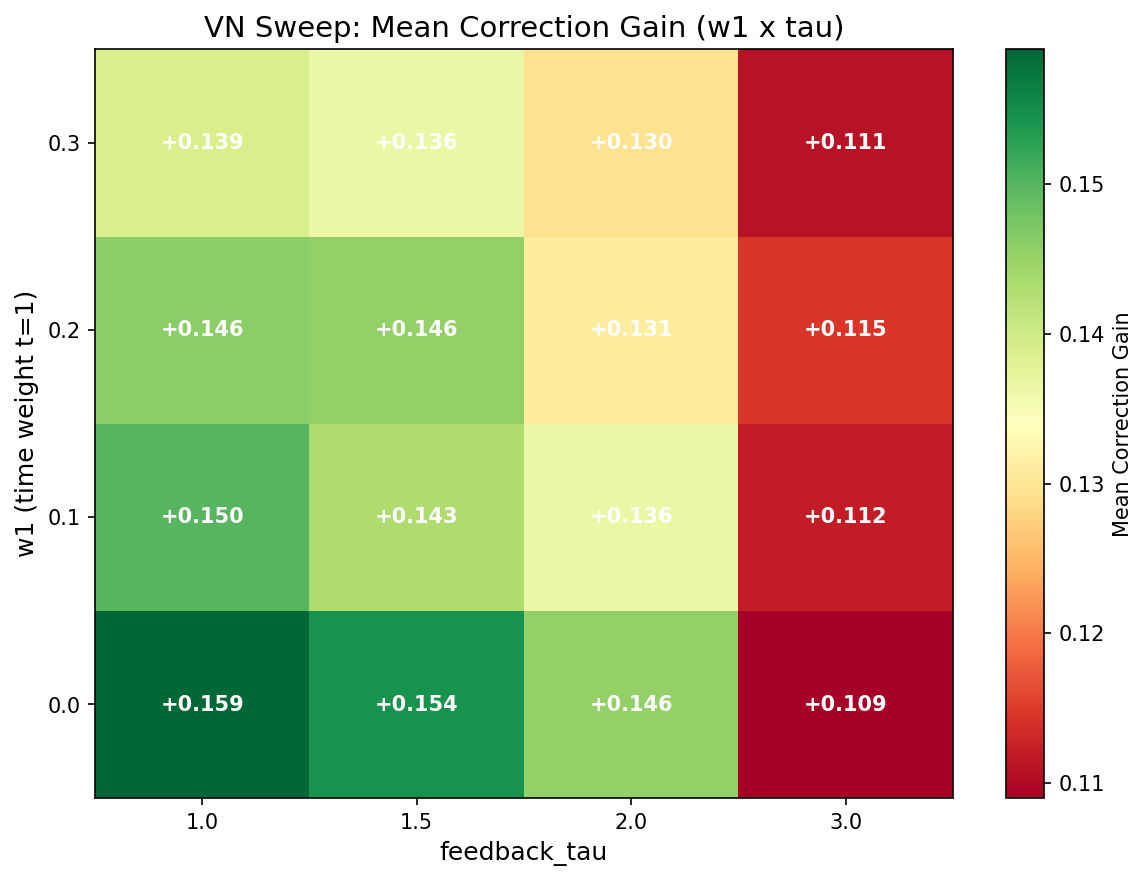
\includegraphics[width=0.8\linewidth]{../results/sweep_vn_heatmap.png}
\caption{VN hyperparameter sweep: mean correction gain across $w_1 \times \tau$ grid. All 16 configurations show positive self-correction (100\% emergence), compared to 68\% under static input.}
\label{fig:vn_sweep}
\end{figure}

\begin{figure}[t]
\centering
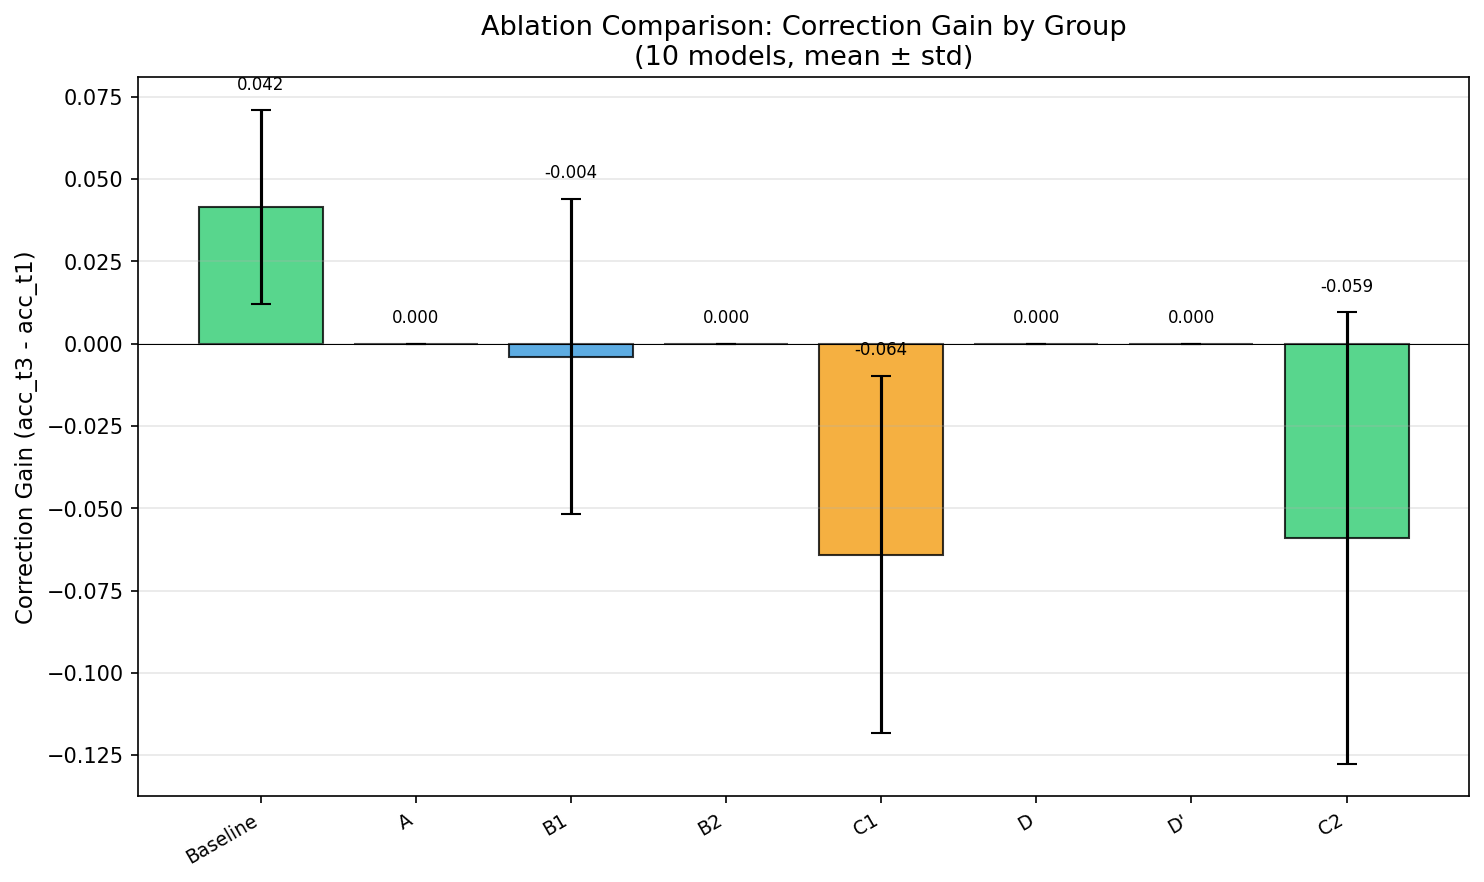
\includegraphics[width=0.8\linewidth]{../results/ablation_comparison.png}
\caption{Correction gain by experimental group at noise level 0.5. Baseline shows positive gain; ablation groups show zero or negative gain. Error bars: $\pm$1 SD across 10 models.}
\label{fig:ablation}
\end{figure}

\subsection{Training Dynamics}
\label{sec:training_dynamics}

To reveal when the feedback contract forms during training, we evaluated Baseline, C1, and C2 correction gain at 11 checkpoints (epoch 0--500) across all 10 models. The contract develops gradually, not abruptly: Baseline gain rises from $\sim$0 at epoch 0 to its final value over $\sim$200 epochs, with no sharp phase transition. C1 (shuffled feedback) gain tracks inversely---as self-correction develops, vulnerability to misaligned feedback increases in parallel (static C1: $+0.018$ at epoch 0 $\to$ $-0.042$ at epoch 500). C2 (clone feedback) harm emerges later than C1 (static C2 turns negative around epoch 100), suggesting that model-specific output geometry takes longer to differentiate than the basic correction mechanism takes to form. Under VN, the same temporal ordering holds with stronger effect sizes.

\subsection{Timestep Extension}
\label{sec:timestep_extension}

To test whether self-correction converges or diverges beyond the training horizon, we extended evaluation to $T \in \{3, 5, 7, 10, 15, 20\}$ on trained models (no retraining). Under both static and variable-noise settings, Baseline accuracy peaked at $T{=}3$ and stabilized thereafter (static: 0.749 at $T{=}3$, 0.741 at $T{=}20$; VN: 0.854 at $T{=}3$, 0.832 at $T{=}20$; evaluated on the timestep-extension test set), consistent with a stable performance plateau over the tested horizons rather than continued refinement or divergence (Figure~\ref{fig:timestep}). Group~A remained flat across all timesteps, confirming no correction without recurrence. Groups C1 and C2 showed slight further degradation at higher $T$ (C1 static: $0.650 \to 0.644$; C1 VN: $0.630 \to 0.615$), confirming that non-veridical feedback compounds rather than self-corrects over additional timesteps.

\begin{figure}[t]
\centering
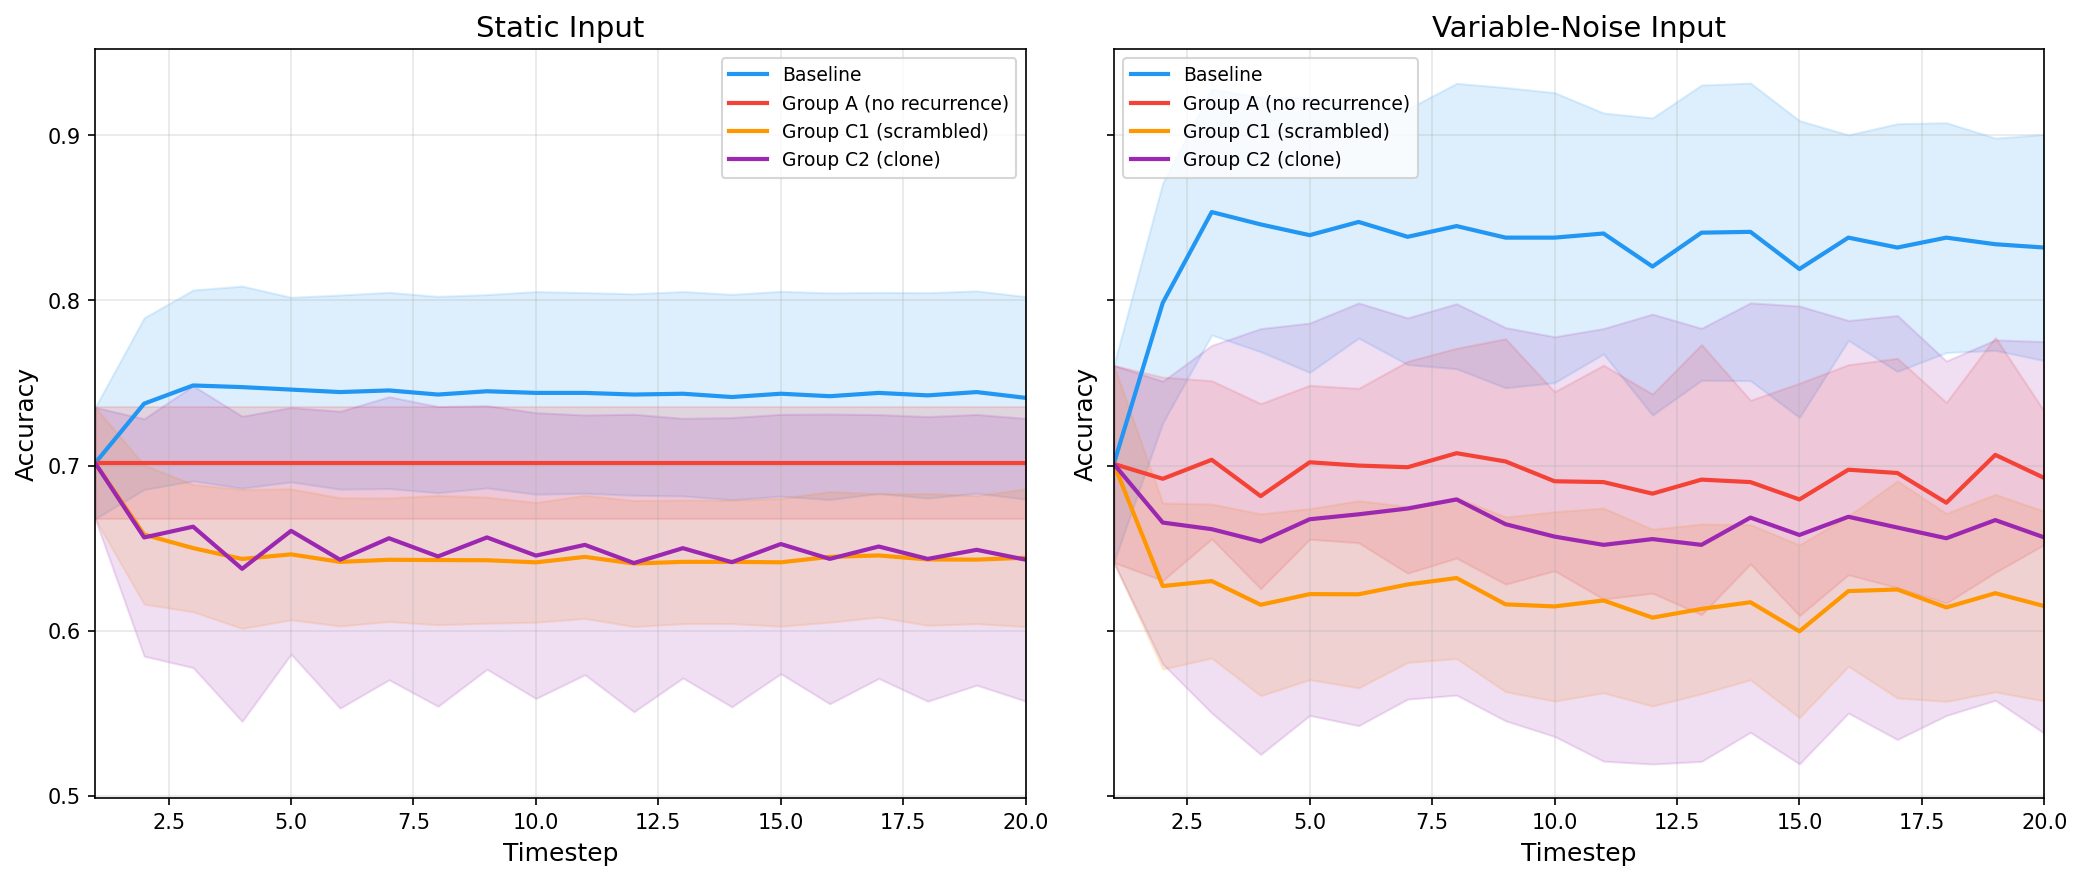
\includegraphics[width=0.8\linewidth]{../results/fig_timestep_extension.png}
\caption{Accuracy vs.\ timestep ($T = 3$--$20$) for static and VN settings. Self-correction converges by $T{=}3$ and stabilizes; ablation groups do not recover at extended timesteps.}
\label{fig:timestep}
\end{figure}

\subsection{Scale Verification}
\label{sec:scale_verification}

To verify that self-correction is not an artifact of the 35-neuron architecture, we tested four hidden-layer widths (10, 20, 45, 245; parameter counts $\sim$325 to $\sim$65,420) on the fixed 5-class task under both static and VN settings. Self-correction (positive Baseline gain) was observed at all scales in both settings (static: $+0.053$ to $+0.033$; VN: $+0.146$ to $+0.149$). Group~A gain was $\approx 0$ at all scales. The C1 fake mirror effect (shuffled feedback is harmful) persisted universally, growing stronger at larger scales (static C1 gain: $-0.044$ at $h{=}10$ to $-0.259$ at $h{=}245$; Figure~\ref{fig:scale}).

C2 (clone feedback) showed a scale-dependent pattern: harmful at small scales ($h{=}10$: $-0.030$, $h{=}20$: $-0.091$ under static) but neutral or slightly beneficial at larger scales under variable noise ($h{=}45$: $+0.032$, $h{=}245$: $+0.060$). This suggests that as model capacity increases, independently trained models may develop more similar output geometries at larger scale, partially satisfying each other's feedback contracts. This scale dependence provides indirect evidence for feedback-contract specificity: at small scales where representations diverge more across random initializations, foreign feedback is harmful; at larger scales where representations converge, it becomes tolerable.

\begin{figure}[t]
\centering
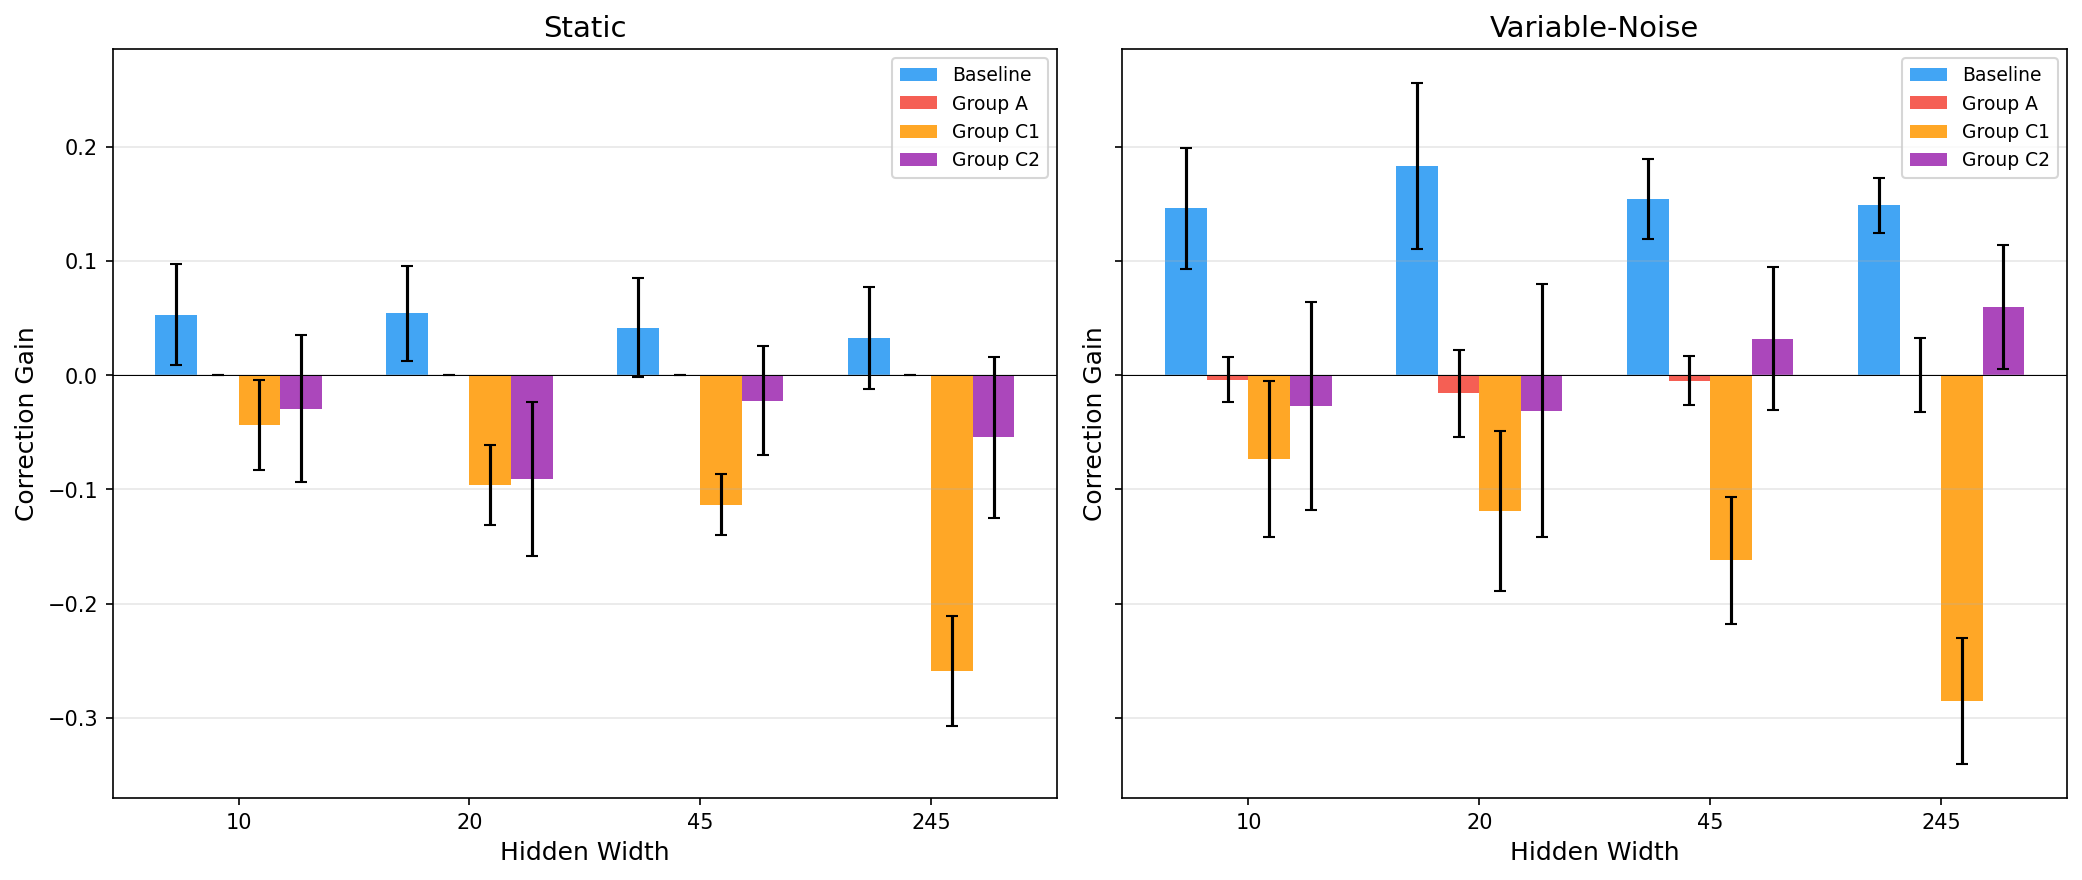
\includegraphics[width=0.8\linewidth]{../results/fig_scale_verification.png}
\caption{Correction gain by hidden-layer width ($h = 10$--$245$) and condition. Self-correction and C1 effects persist at all scales; C2 harm diminishes at larger scales under VN.}
\label{fig:scale}
\end{figure}

\subsection{MNIST Extension}
\label{sec:mnist}

To test whether the core findings generalize beyond the synthetic 5-class task, we replicated the experiment on MNIST (10-class, 784-dimensional input) using the same RecurrentMLP architecture scaled to Input(784) $\to$ H1(128) $\to$ H2(128) $\to$ Output(10) with output$\to$hidden feedback ($\sim$130k parameters). Ten target models (seeds 0--9) and ten donors (seeds 100--109) were trained for 30 epochs with SGD ($\text{lr}{=}0.01$) under variable noise ($\sigma = 0.5$, $T = 3$) with the same time-weighted loss ($w_1 = 0.0$, $w_2 = 0.2$).

Self-correction replicated: Baseline gain $= +0.021 \pm 0.003$ (all 10 models positive, $p = 0.002$ vs.\ Group~A). Group~A gain $= -0.001 \pm 0.002$---removing recurrent feedback eliminated correction. The C1 fake mirror effect also replicated clearly: C1 gain $= -0.019 \pm 0.018$ ($p = 0.002$ vs.\ Baseline), confirming that shuffled feedback is actively harmful even on a real-world dataset.

C2 (clone feedback) showed gain $= +0.006 \pm 0.007$---positive, unlike the negative C2 gain observed in the 35-neuron model. Clone feedback was not harmful on MNIST but was still significantly worse than self-feedback (Baseline $-$ C2 $= +0.015$, $p = 0.002$). This is consistent with the scale-dependent C2 pattern observed in \S\ref{sec:scale_verification}: at 130k parameters, independently trained models develop sufficiently similar representations that clone feedback provides partial but suboptimal correction. The dissociation between C1 (harmful) and C2 (suboptimal but not harmful) at this scale is itself informative---it demonstrates that the fake mirror effect is driven by coordinate disruption (C1), not merely by foreign-model identity (C2).

Training dynamics on MNIST reveal a contrast with the 35-neuron model: self-correction emerges within the first epoch (Baseline gain $+0.012$ at epoch 1) and C1 harm appears simultaneously ($-0.016$), whereas in the 35-neuron model both develop over $\sim$200 epochs. Most notably, C2 is initially harmful at epoch 1 ($-0.035$) but recovers to positive by epoch 3 as model representations converge during training. This inverted C2 trajectory---harmful early, tolerable late---provides direct evidence that feedback-contract specificity reflects representation divergence between models, which is maximal in early training and diminishes as models converge toward similar solutions.

% ============================================================
\section{Discussion}
% ============================================================

\subsection{Induction Depends on Conditions, Not Merely Scale}

Self-correction developed in a network of 35 neurons---orders of magnitude smaller than systems where iterative refinement is typically studied. What mattered was not scale but two learning conditions: temporal freedom and gradient flow through the feedback pathway. Under VN, Group~A gain $\approx 0$ ($p = 0.754$) is the expected statistical baseline for a stateless model under i.i.d.\ inputs; the informative result is the Baseline's gain of $+0.151$, demonstrating evidence accumulation through recurrent feedback.

One might argue that VN self-correction is simply Bayesian evidence accumulation. The VN setting does provide independent observations that a temporal integrator can exploit, and the larger VN gain ($+0.151$ vs.\ $+0.042$ static) is consistent with an evidence-accumulation component. The key point is that this accumulation requires a mechanism for temporal integration: stateless models (Group~A, D, D$'$, D$''$) have expected gain of zero under i.i.d.\ inputs and show gain $\approx 0$ empirically. VN self-correction likely involves both evidence accumulation and error revision, both of which depend on recurrent self-reference in our setting.

\subsection{The Fake Mirror Is Worse Than No Mirror}

The ``fake mirror'' effect---non-veridical feedback degrades performance below the no-feedback baseline---is clearly demonstrated under static input (C1 vs A: corrected $p = 0.008$; C2 vs A: corrected $p = 0.065$, marginally non-significant) and directionally consistent under VN. C2 harm attenuates under VN ($-0.018$ vs.\ $-0.059$ under static), likely because the clone's output varies across timesteps in response to different noise realizations, producing less systematic misdirection. This suggests that the feedback contract's influence scales with the network's reliance on self-generated signals.

An important caveat is that the C2 clone-feedback effect is scale-dependent. At hidden width $\geq 45$ under variable noise, clone feedback becomes neutral or slightly positive (\S\ref{sec:scale_verification}), and on MNIST (130k parameters) C2 gain is positive though still significantly below self-feedback (\S\ref{sec:mnist}). This pattern is itself consistent with feedback-contract specificity: at small scales where independently trained models develop more divergent representations, foreign feedback violates the learned contract; at larger scales where representations converge, the contract is partially satisfied. The core phenomena---self-correction, the C1 fake mirror effect, and the superiority of self-feedback over clone feedback---persist at all tested scales.

The interpolation sweep (\S\ref{sec:interpolation_results}) extends this to a continuous mapping: smooth degradation with zero-crossing at $\alpha \approx 0.2$--$0.3$ reveals a ``soft'' feedback contract. The mechanistic analysis (\S\ref{sec:geometry_results}) provides geometric evidence: self and clone $W_\text{rec}$ contributions diverge by 0.73 (vs.\ 0.36 for same-class resampled self, 1.00 for random), and higher divergence correlates with greater C2 degradation ($\rho = -0.61$, $p = 0.062$). This divergence persists even when self and clone agree on the predicted class, indicating that feedback-contract specificity operates at the continuous geometry level. Moderate $W_\text{rec}$ sign consistency across seeds (0.614) suggests that each model develops a distinct geometric signature for interpreting feedback. The affine alignment control (\S\ref{sec:geometry_results}) provides a quantitative decomposition: approximately 60\% of C2 degradation is attributable to linear representation misalignment (recoverable by a learned affine transform), while the remaining ${\sim}40\%$ persists after optimal linear correction---confirming that feedback-contract specificity has a genuinely non-linear component beyond simple covariate shift.

\subsection{Implications for AI Systems}

Extrapolation from toy models to billion-parameter systems requires caution, but the MNIST extension (\S\ref{sec:mnist}) provides a partial bridge: self-correction and the C1 fake mirror effect replicate at 130k parameters on a real-world dataset. The C2 effect is scale-dependent---harmful at small scales, suboptimal but not harmful at MNIST scale---suggesting that feedback-contract specificity is strongest when model representations are most individualized. The core finding that recurrent self-reference is necessary for correction (Group~A $\approx 0$ in all settings) is consistent with theoretical arguments that self-referential structure is representationally necessary for certain forms of meta-learning \citep{kirsch2022eliminating}. The C1 result---that misaligned feedback is worse than no feedback---is a cautionary observation for any system that trains on external signals as if they were self-generated: feedback that deviates from the model's own output geometry may actively degrade rather than merely fail to improve. Whether this applies to RLHF or preference-based training at scale is an open empirical question that this minimal study cannot answer, but the direction of the effect is consistent across all scales we tested. A natural next step would be testing whether distillation from a foreign reward model produces measurably different alignment dynamics than self-generated reward, adapting the interpolation methodology (\S\ref{sec:interpolation}) to the RLHF setting.

\subsection{Connection to Biological Metacognition}

The partially overlapping neurons serving both pattern recognition and self-correction in our model bear a surface-level resemblance to overlapping monitoring and control circuits in prefrontal cortex \citep{morales2018domain}. However, this analysis was exploratory (single model, seed=0) and the toy setting precludes strong conclusions about biological relevance.

\subsection{Relationship to Chain-of-Thought and Test-Time Compute}

Our time-weighted loss is analogous in one respect to Chain-of-Thought prompting \citep{wei2022chain}: both reduce pressure on intermediate computation steps, granting the model additional processing without penalizing intermediate exploration. Unlike PonderNet or ACT, our approach requires no explicit halting mechanism---only a loss reweighting.

\subsection{Limitations}

\begin{enumerate}

\item \textbf{Induced, not spontaneous.} Self-correction was induced by the time-weighted loss, which explicitly removes penalty for early errors. This is a learned behavior requiring specific training conditions, not a spontaneous capability.

\item \textbf{Toy system.} Thirty-five neurons performing pattern classification cannot capture the complexity of language or reasoning. The variable-noise task adds ecological validity but does not replicate the entangled memory-and-correction demands of autoregressive systems. The value of our experiment lies in its mechanistic transparency, not its ecological validity. The Hodgkin--Huxley analogy (\S1.2) is intended methodologically: the value of the preparation lies in enabling measurement techniques, not in claiming that 35-neuron dynamics will recapitulate in all larger systems. The MNIST extension (\S\ref{sec:mnist}) provides a partial bridge, but a substantial gap remains between 130k parameters and the scales at which iterative refinement is practically deployed.

\item \textbf{Modest effect size.} The correction gain ($+0.042$ static, $+0.151$ variable noise) is small in absolute terms. The parameter-matched feedforward model (D$'$) achieves higher absolute accuracy ($0.822$) than the recurrent Baseline at $t{=}3$ ($0.739$), representing a different computational trade-off: one-shot optimization vs.\ progressive refinement through self-reference. Under capacity constraints where single-pass accuracy is insufficient, the recurrent strategy may prove essential.

\item \textbf{Mechanistic specificity.} The mechanistic analysis (trajectory visualization, $W_\text{rec}$ dissection, cosine divergence) is specific to this 35-neuron architecture. Whether the same geometric signatures of feedback-contract specificity appear in larger recurrent architectures is untested.

\item \textbf{Statistical power.} $N{=}10$ models bounds the minimum achievable $p$-value ($\sim$0.002 before correction), limiting detection of subtle effect-size differences---for example, the C1-vs-C2 and C2-vs-zero comparisons under variable noise. The interpolation sweep partially compensates by providing continuous evidence, but individual point comparisons remain power-limited.

\item \textbf{Partial alignment recovery.} The learned affine alignment control (\S\ref{sec:geometry_results}) recovers ${\sim}60\%$ of C2 degradation, indicating that a substantial portion of clone-feedback harm at the 35-neuron scale reflects linear representation misalignment rather than deeper geometric incompatibility. The remaining ${\sim}40\%$ persists after optimal linear correction ($p < 0.01$ under VN), but whether a non-linear alignment (e.g., a small neural network mapping donor logits to target logits) would recover more remains untested. If non-linear alignment fully rescues performance, feedback-contract specificity reduces entirely to representation divergence---still a valid finding, but a weaker claim than model-specific geometric incompatibility.

\end{enumerate}

% ============================================================
\section{Conclusion}
% ============================================================

In a 35-neuron recurrent network, we have mechanistically dissected learned feedback-contract specificity---the co-adaptation of recurrent weights to a model's own output geometry. Six lines of evidence converge:

\begin{enumerate}

\item \textbf{Variable-noise task} provides independent noisy observations at each timestep, enabling evidence accumulation: the recurrent Baseline achieves gain $= +0.151$, while Group~A (gain $\approx 0$, as expected for a stateless model under i.i.d.\ inputs) and stateless feedforward controls confirm that input variation alone, without recurrent feedback, is insufficient.

\item \textbf{Feedback interpolation} maps a smooth, monotonic degradation from full self-feedback (gain $= +0.053$) to full contamination (gain $\leq 0$), with the zero-crossing at $\alpha \approx 0.2$--$0.3$---indicating a soft but model-specific feedback contract.

\item \textbf{Hidden-state trajectory analysis, wrong-trajectory control, and affine alignment} show corrected trials converging toward class centroids under self-feedback but diverging under clone feedback, with mean cosine divergence of 0.73 (0.36 resampled self, 1.00 random). The wrong-trajectory control confirms that the degradation is model-specific: same-model different-trial feedback preserves correction ($p = 0.002$ under VN), while foreign-model feedback degrades it. A learned affine alignment recovers ${\sim}60\%$ of the C2 degradation but leaves a significant residual ($p < 0.01$ under VN), decomposing the feedback contract into a linearly correctable component (${\sim}60\%$) and a non-linear model-specific residual (${\sim}40\%$).

\item \textbf{Ablation and control experiments} confirm that neither parameters (D$'$), computational depth (D$''$), nor valid-but-foreign feedback (C2) can substitute for the model's own output. These findings hold across 68\% of 80 static hyperparameter configurations and 100\% of 16 VN configurations.

\item \textbf{Scale verification} across hidden widths 10--245 confirms that self-correction and the C1 fake mirror effect persist regardless of model capacity. C2 clone feedback shows scale-dependent harm---negative at small scales, neutral at large scales under variable noise---consistent with representation convergence at higher capacity.

\item \textbf{MNIST extension} (784-dim input, 130k parameters, 10-class) replicates self-correction ($+0.021$) and the C1 fake mirror effect ($-0.019$), while C2 clone feedback is suboptimal but not harmful ($+0.006$), consistent with the scale-dependent pattern.

\end{enumerate}

The central finding is that feedback utility is graded by geometric compatibility: self-feedback produces the largest correction, clone feedback is intermediate (with the gap modulated by representation convergence across scale), and shuffled feedback actively degrades performance. This graded structure---not a binary ``works/doesn't work''---provides a candidate diagnostic for studying output-feedback processing in neural systems. We offer these results as a mechanistic case study from a fully transparent minimal model. Whether the same feedback-fidelity dependence manifests in large-scale systems trained with external feedback signals---where the gap between the feedback source and the model's own output geometry may be substantial---is a question for larger-scale studies than this independent effort can provide.

% ============================================================
\section*{Data Availability}
% ============================================================

All code, data, and analysis scripts will be publicly released upon acceptance. The experiment is implemented in pure NumPy and can be reproduced on a standard multi-core desktop computer. The core experiments (static and variable-noise ablation) complete in under one hour; the full pipeline including hyperparameter sweeps and mechanistic analyses requires approximately 4--6 hours with parallelization. Raw experimental data (12,850 rows across 12 CSV files covering all conditions) are included.

% ============================================================
\section*{Author Contributions}
% ============================================================

The author designed and implemented all experiments, executed all analyses, and wrote the manuscript.

% ============================================================
\section*{Acknowledgments}
% ============================================================

The experimental design was iteratively refined through structured dialogue with large language models---Claude Opus 4.6 (Anthropic), GPT-5.4 Pro (OpenAI), and Gemini Deep Think (Google)---which served as critical reviewers identifying methodological gaps and suggesting additional controls. The author takes full responsibility for all scientific claims and interpretations.

% ============================================================
\section*{Conflict of Interest}
% ============================================================

The author declares no conflict of interest. This research was conducted independently without institutional or corporate funding.

% ============================================================
\section*{Ethics Statement}
% ============================================================

This work studies fundamental mechanisms of iterative refinement in a minimal artificial neural network. The system is a 35-neuron toy model performing synthetic pattern classification; it has no direct real-world application and poses no foreseeable societal risk. The research may contribute to longer-term understanding of self-referential processing in AI systems, which is relevant to AI safety and alignment research. No human subjects were involved. All experiments are fully reproducible from the publicly available code and data.

\bibliography{references}
\bibliographystyle{tmlr}

% ============================================================
\appendix
\section{Additional Figures}
% ============================================================

\begin{figure}[h]
\centering
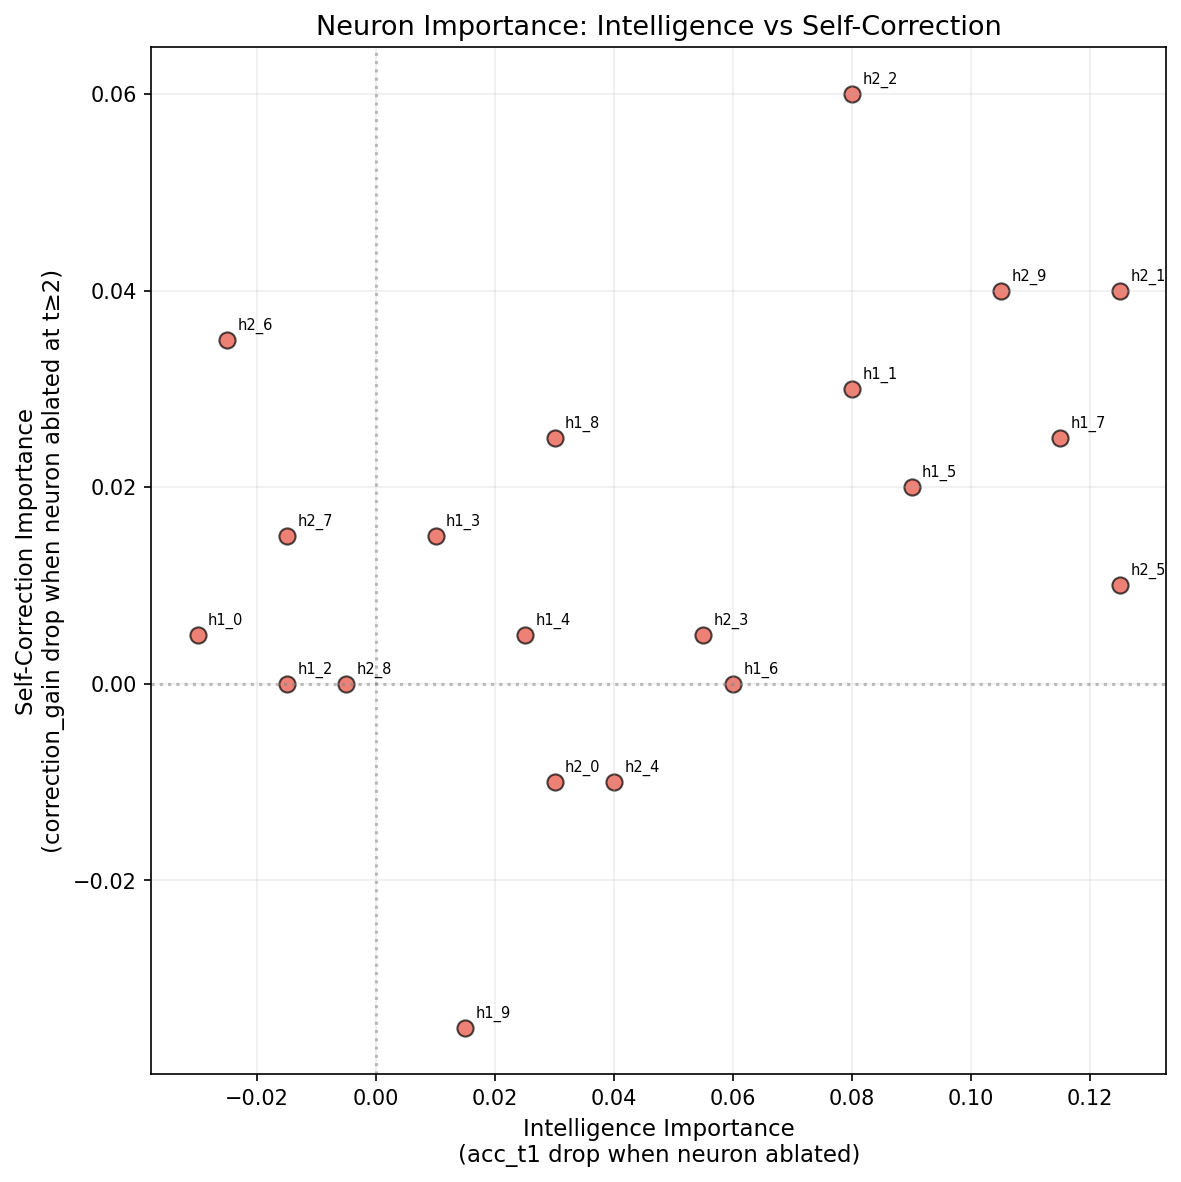
\includegraphics[width=0.7\linewidth]{../results/neuron_importance_heatmap.png}
\caption{Neuron importance: intelligence (feedforward) vs.\ correction (recurrent) contribution. Exploratory analysis on a single model (seed=0).}
\label{fig:neuron}
\end{figure}

\begin{figure}[h]
\centering
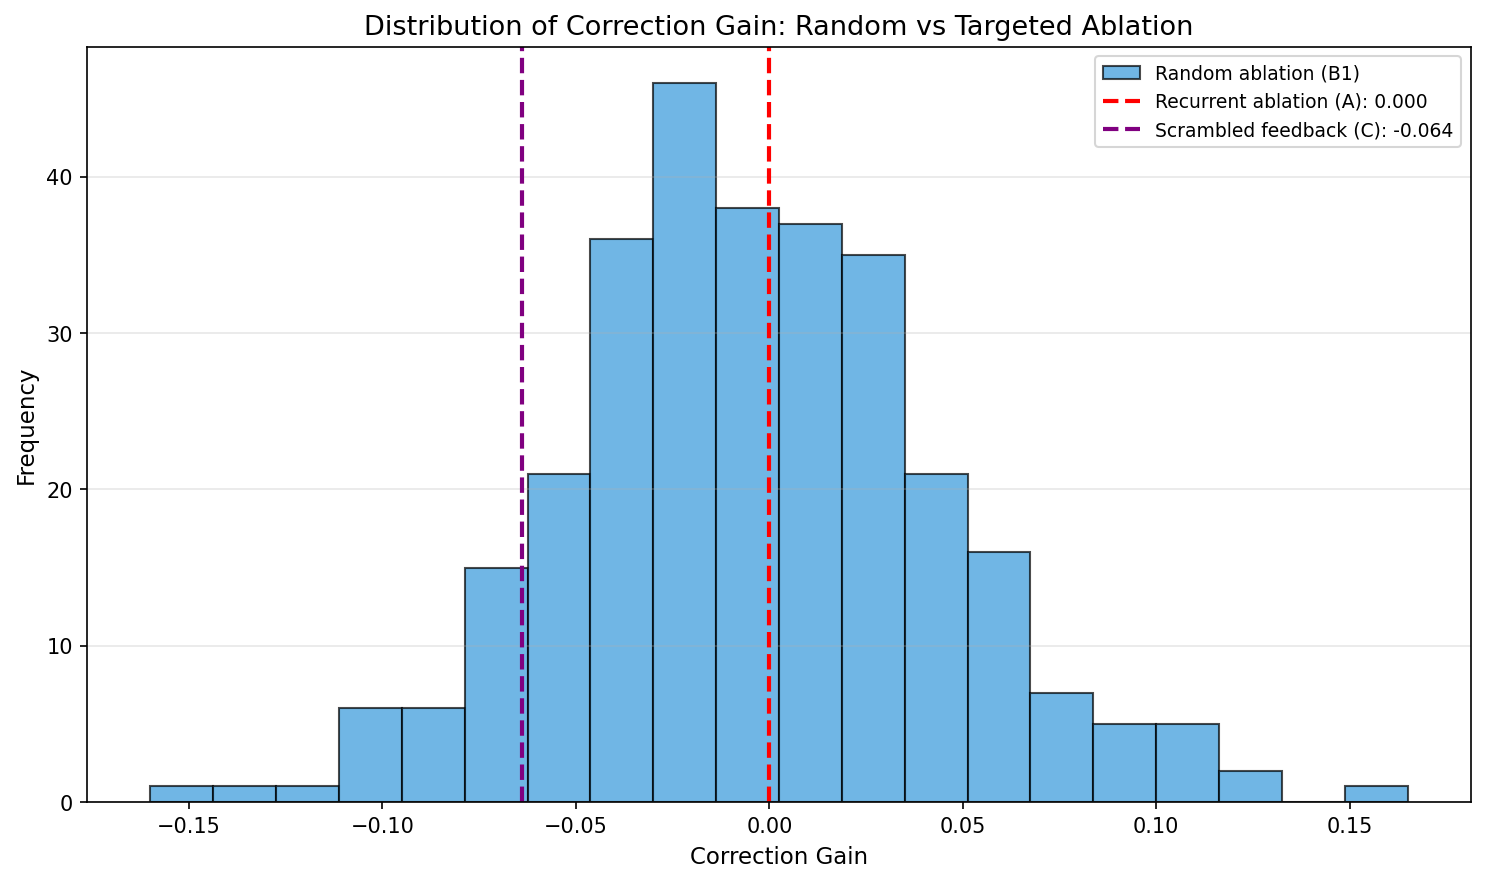
\includegraphics[width=0.7\linewidth]{../results/accuracy_distribution.png}
\caption{Distribution of correction gain under random ablation (Group~B1, 30 repeats $\times$ 10 models). Vertical lines show Group~A and Group~C1 positions for comparison.}
\label{fig:distribution}
\end{figure}

\end{document}
